% ============================================================
% AAK Academy Management System - Database Design Document
% Namal University | Database Systems | June 2026
% ============================================================

\documentclass[12pt,a4paper]{report}

% ---- Packages ----
\usepackage[a4paper, margin=1in, top=1.2in, bottom=1.2in]{geometry}
\usepackage{fontenc}
\usepackage{inputenc}
\usepackage{times}           % Times New Roman
\usepackage{setspace}
\usepackage{titlesec}
\usepackage{tocloft}
\usepackage{graphicx}
\usepackage{float}
\usepackage{booktabs}
\usepackage{longtable}
\usepackage{array}
\usepackage{tabularx}
\usepackage{multirow}
\usepackage{xcolor}
\usepackage{listings}
\usepackage{fancyhdr}
\usepackage{hyperref}
\usepackage{caption}
\usepackage{parskip}
\usepackage{enumitem}
\usepackage{makecell}
\usepackage{amsmath}
\usepackage[T1]{fontenc}

% ---- Colors ----
\definecolor{codegreen}{rgb}{0,0.5,0}
\definecolor{codegray}{rgb}{0.5,0.5,0.5}
\definecolor{codebg}{rgb}{0.97,0.97,0.97}
\definecolor{darkgreen}{RGB}{26,71,49}
\definecolor{goldcolor}{RGB}{201,162,39}

% ---- Hyperref Setup ----
\hypersetup{
    colorlinks=true,
    linkcolor=darkgreen,
    urlcolor=darkgreen,
    citecolor=darkgreen,
    pdfborder={0 0 0}
}

% ---- Code Listings ----
\lstset{
    backgroundcolor=\color{codebg},
    basicstyle=\ttfamily\footnotesize,
    breakatwhitespace=false,
    breaklines=true,
    captionpos=b,
    commentstyle=\color{codegreen},
    keepspaces=true,
    keywordstyle=\color{blue}\bfseries,
    language=SQL,
    numbers=left,
    numbersep=5pt,
    numberstyle=\tiny\color{codegray},
    showspaces=false,
    showstringspaces=false,
    showtabs=false,
    stringstyle=\color{red},
    tabsize=2,
    frame=single,
    rulecolor=\color{gray!40},
    xleftmargin=10pt,
    xrightmargin=5pt,
}

% ---- Heading Styles (matching Namal template) ----
% Chapter (Level 1): TNR 18pt, ALLCAPS, right-aligned
\titleformat{\chapter}[block]
  {\fontsize{18}{22}\selectfont\bfseries\MakeUppercase\raggedleft}
  {CHAPTER \thechapter:}{0.5em}{}
\titlespacing*{\chapter}{0pt}{20pt}{20pt}

% Section (Level 2): TNR 16pt, ALLCAPS, left-aligned
\titleformat{\section}
  {\fontsize{16}{20}\selectfont\bfseries\MakeUppercase}
  {\thesection.}{0.5em}{}
\titlespacing*{\section}{0pt}{14pt}{8pt}

% Subsection (Level 3): TNR 14pt, Title Case, left-aligned
\titleformat{\subsection}
  {\fontsize{14}{18}\selectfont\bfseries}
  {\thesubsection.}{0.5em}{}
\titlespacing*{\subsection}{0pt}{10pt}{6pt}

% ---- Table of Contents Formatting ----
\renewcommand{\cftchapfont}{\bfseries}
\renewcommand{\cftsecfont}{}
\setlength{\cftbeforechapskip}{6pt}

% ---- Page Style ----
\pagestyle{fancy}
\fancyhf{}
\fancyhead[L]{\small AAK Academy Management System}
\fancyhead[R]{\small Namal University}
\fancyfoot[C]{\thepage}
\renewcommand{\headrulewidth}{0.4pt}

% ---- Paragraph Spacing ----
\setlength{\parskip}{8pt}
\setlength{\parindent}{0pt}

% ---- Table column types ----
\newcolumntype{L}[1]{>{\raggedright\arraybackslash}p{#1}}
\newcolumntype{C}[1]{>{\centering\arraybackslash}p{#1}}

% ============================================================
\begin{document}

% ============================================================
%  TITLE PAGE
% ============================================================
\begin{titlepage}
\centering
{\fontsize{20}{24}\selectfont\bfseries AAK ACADEMY MANAGEMENT SYSTEM (AAMS)\par}
\vspace{0.5cm}
{\fontsize{16}{20}\selectfont\bfseries Database Design Document\par}
\vspace{0.3cm}
{\large V 2.0\par}

{\large \textbf{By}\par}
\vspace{0.5cm}

\begin{tabular}{|c|l|l|}
\hline
\textbf{Sr.} & \textbf{Group Member Name} & \textbf{Roll No.} \\
\hline
1 & SALMAN SAFDAR & NUM-BSCS-2024-70 \\
2 & MUHAMMAD HARIS & NUM-BSCS-2024-49 \\
3 & FARWA IMRAN & NUM-BSCS-2024-22 \\
\hline
\end{tabular}

\vspace{2cm}
\begin{figure}
            \centering
            \includegraphics[width=1\linewidth]{}
\begin{figure}
                \centering
                
\includegraphics[width=0.4\linewidth]{namallogo.png}
            \end{figure}
                        \label{fig:placeholder}
        \end{figure}

{\large\textbf{Department of Computer Sciences}\par}
\vspace{0.3cm}
{\large\textbf{Namal University, Mianwali, Pakistan}\par}
\vspace{0.5cm}
{\large\textbf{Submission Date: 21\textsuperscript{st} June, 2026}\par}

\vfill

\begin{tabular}{|l|l|}
\hline
\textbf{Course} & Database Systems \\
\hline
\textbf{Database Name} & aak\_academy \\
\hline
\textbf{DBMS} & MySQL 8.x \\
\hline
\textbf{Frontend} & HTML5, CSS3, JavaScript \\
\hline
\textbf{Backend} & Node.js, Express.js \\
\hline
\textbf{Database Driver} & mysql2 (connection pool) \\
\hline
\textbf{GitHub} & \href{https://github.com/bscs24f22-eng/DataBase-Project}{github.com/bscs24f22-eng/DataBase-Project} \\
\hline
\end{tabular}

\end{titlepage}

% ============================================================
%  REVISION HISTORY
% ============================================================
\thispagestyle{plain}
{\large\bfseries REVISION HISTORY\par}
\vspace{0.5cm}

\begin{tabularx}{\textwidth}{|C{2cm}|C{2cm}|X|C{3cm}|}
\hline
\textbf{Date} & \textbf{Version} & \textbf{Description} & \textbf{Approved By} \\
\hline
21/06/26 & V 2.0 & Final submission with full implementation, GUI, and database connectivity & \\
\hline
15/05/26 & V 1.0 & Initial ERD, conceptual design, relational schema draft & \\
\hline
\end{tabularx}

\newpage

% ============================================================
%  TABLE OF CONTENTS
% ============================================================
\tableofcontents
\newpage

% ============================================================
%  CHAPTER 1: PROJECT OVERVIEW
% ============================================================
\chapter{PROJECT OVERVIEW}

\section{INTRODUCTION}

The \textbf{AAK Academy Management System (AAMS)} is a web-based academic management application developed for AAK Academy at Namal University. The system centralizes academic, financial, and communication operations for three user roles: \textbf{Admin}, \textbf{Teacher}, and \textbf{Student}.

Previously, the application used static in-memory JavaScript data. This project implements a \textbf{full three-tier architecture} with a MySQL relational database, RESTful API backend, and role-based web GUI. All CRUD operations persist to the database in real time, enabling reliable and consistent data management across the entire academy.

The system is built to support the real-world scenario of an educational institution that manages large volumes of interconnected data including student records, course enrollments, assessments, attendance, and financial transactions.

\section{PROBLEM STATEMENT}

Educational institutions manage large volumes of interconnected data — students, courses, enrollments, fees, assignments, quizzes, attendance, and announcements. Manual or disconnected systems lead to several critical problems:

\begin{itemize}[noitemsep]
    \item \textbf{Data Inconsistency:} The same information stored in multiple places leads to conflicting records.
    \item \textbf{Data Duplication:} Redundant entries waste storage and create maintenance challenges.
    \item \textbf{Poor Traceability:} Without audit logs, it is difficult to track who changed what and when.
    \item \textbf{Lack of Role Separation:} Static systems do not enforce access control based on user roles.
    \item \textbf{Manual Financial Tracking:} Fee collection, payment records, and discount management are error-prone when done manually.
    \item \textbf{No Real-Time Updates:} In-memory data is lost on server restart and cannot persist across sessions.
\end{itemize}

The AAMS system addresses all of these challenges through a normalized relational database with proper constraints, referential integrity, and a role-based access control model.

\section{PROJECT OBJECTIVES}

\textbf{General Objective:} To develop a fully functional, database-driven academic management system that centralizes all administrative, academic, and financial operations of AAK Academy into a secure, consistent, and scalable platform.

\textbf{Specific Objectives:}

\begin{itemize}[noitemsep]
    \item Design a normalized relational database schema satisfying 3NF/BCNF. \hfill \textbf{[Completed]}
    \item Convert the ERD entities into MySQL tables with proper constraints. \hfill \textbf{[Completed]}
    \item Populate the database with realistic sample data using DML scripts. \hfill \textbf{[Completed]}
    \item Build a role-based GUI for Admin, Teacher, and Student users. \hfill \textbf{[Completed]}
    \item Connect the GUI to MySQL via a RESTful API using Node.js. \hfill \textbf{[Completed]}
    \item Support real-time CRUD operations that persist immediately to the database. \hfill \textbf{[Completed]}
    \item Maintain referential integrity, cascade deletes, and audit logging. \hfill \textbf{[Completed]}
\end{itemize}

\textbf{GitHub Repository:} \href{https://github.com/bscs24f22-eng/DataBase-Project}{https://github.com/bscs24f22-eng/DataBase-Project}

% ============================================================
%  CHAPTER 2: CONCEPTUAL DATABASE DESIGN
% ============================================================
\chapter{CONCEPTUAL DATABASE DESIGN}

\section{ENTITY}

The following entities are identified as the core components of the AAMS database. Associative/junction entities are not listed here as they emerge from many-to-many relationships.

\begin{longtable}{|C{1.2cm}|L{3.5cm}|L{9cm}|}
\hline
\textbf{Sr.} & \textbf{Entity Name} & \textbf{Description} \\
\hline
\endfirsthead
\hline
\textbf{Sr.} & \textbf{Entity Name} & \textbf{Description} \\
\hline
\endhead
01 & USER & An individual registered in the system with a login identity and an assigned role (Admin, Teacher, or Student). \\
\hline
02 & ADMIN & A privileged user with full system access who manages all academic and financial records. \\
\hline
03 & TEACHER & An academic user responsible for managing subjects, assessments, attendance, and materials. \\
\hline
04 & STUDENT & An enrolled learner who participates in subjects, submits assignments, and views academic records. \\
\hline
05 & PROGRAM & An academic degree or diploma programme offered by the institution. \\
\hline
06 & SUBJECT & A course taught within a programme, assigned to a specific teacher. \\
\hline
07 & ASSIGNMENT & A task created by a teacher for students in a subject, with a deadline and marks. \\
\hline
08 & QUIZ & A timed online assessment created by a teacher for a specific subject. \\
\hline
09 & QUIZ\_QUESTION & An individual question belonging to a quiz. \\
\hline
10 & LIVE\_CLASS & A scheduled online session with a Zoom link, date, and time managed by a teacher. \\
\hline
11 & LEARNING\_MATERIAL & A file or document uploaded by a teacher for students of a subject. \\
\hline
12 & ANNOUNCEMENT & A notice posted by a teacher or admin relevant to a subject or the whole academy. \\
\hline
13 & FEE\_RECORD & A financial record tracking total fees, discounts, payments, and balance for a student. \\
\hline
14 & PAYMENT & An individual payment transaction made against a student's fee record. \\
\hline
15 & NOTIFICATION & A system-generated message sent to a user. \\
\hline
16 & AUDIT\_LOG & A security log recording all significant actions performed by users in the system. \\
\hline
\end{longtable}

\section{DATA DICTIONARY}

\subsection{USER}

\begin{longtable}{|C{1cm}|L{3cm}|L{2.5cm}|L{2.5cm}|L{5cm}|}
\hline
\textbf{Sr.} & \textbf{Name} & \textbf{Data Type} & \textbf{Constraint} & \textbf{Description} \\
\hline
\endfirsthead
\hline
\textbf{Sr.} & \textbf{Name} & \textbf{Data Type} & \textbf{Constraint} & \textbf{Description} \\
\hline
\endhead
01 & user\_id (PK) & INT & NOT NULL, AUTO\_INCREMENT & Unique identifier for each user \\
\hline
02 & full\_name & VARCHAR(100) & NOT NULL & Full name of the user \\
\hline
03 & email & VARCHAR(100) & NOT NULL, UNIQUE & Login email address \\
\hline
04 & password\_hash & VARCHAR(255) & NOT NULL & Hashed password for authentication \\
\hline
05 & role & ENUM & NOT NULL & Role: admin, teacher, or student \\
\hline
06 & phone & VARCHAR(20) & NULL & Contact phone number \\
\hline
07 & status & ENUM & DEFAULT 'active' & Account status: active or inactive \\
\hline
08 & created\_at & DATETIME & DEFAULT NOW() & Timestamp of account creation \\
\hline
\end{longtable}

\subsection{STUDENT}

\begin{longtable}{|C{1cm}|L{3cm}|L{2.5cm}|L{2.5cm}|L{5cm}|}
\hline
\textbf{Sr.} & \textbf{Name} & \textbf{Data Type} & \textbf{Constraint} & \textbf{Description} \\
\hline
\endfirsthead
\hline
\textbf{Sr.} & \textbf{Name} & \textbf{Data Type} & \textbf{Constraint} & \textbf{Description} \\
\hline
\endhead
01 & student\_id (PK) & INT & NOT NULL, AUTO\_INCREMENT & Unique identifier for each student \\
\hline
02 & user\_id & INT & NOT NULL, UNIQUE & Reference to USER table \\
\hline
03 & dob & DATE & NULL & Date of birth \\
\hline
04 & gender & ENUM & NULL & Gender: male, female, or other \\
\hline
05 & program\_id & INT & FK, NULL & Programme the student is enrolled in \\
\hline
06 & enrollment\_date & DATE & NULL & Date of initial enrolment \\
\hline
07 & fee\_status & ENUM & DEFAULT 'unpaid' & Current fee status: paid, unpaid, partial \\
\hline
\end{longtable}

\subsection{SUBJECT}

\begin{longtable}{|C{1cm}|L{3cm}|L{2.5cm}|L{2.5cm}|L{5cm}|}
\hline
\textbf{Sr.} & \textbf{Name} & \textbf{Data Type} & \textbf{Constraint} & \textbf{Description} \\
\hline
\endfirsthead
\hline
\textbf{Sr.} & \textbf{Name} & \textbf{Data Type} & \textbf{Constraint} & \textbf{Description} \\
\hline
\endhead
01 & subject\_id (PK) & INT & NOT NULL, AUTO\_INCREMENT & Unique identifier for the subject \\
\hline
02 & program\_id & INT & FK, NULL & Programme this subject belongs to \\
\hline
03 & teacher\_id & INT & FK, NULL & Teacher assigned to this subject \\
\hline
04 & subject\_name & VARCHAR(100) & NOT NULL & Name of the subject \\
\hline
05 & credit\_hours & INT & NOT NULL & Credit hours assigned \\
\hline
06 & fee & DECIMAL(10,2) & NOT NULL & Fee charged for this subject \\
\hline
07 & prerequisite & VARCHAR(100) & NULL & Name of any prerequisite subject \\
\hline
\end{longtable}

\section{BUSINESS RULES}

\begin{itemize}[noitemsep]
    \item A user must have exactly one role: Admin, Teacher, or Student.
    \item A student can enroll in multiple subjects; a subject can have multiple students enrolled (M:N via enrollment table).
    \item A student belongs to exactly one programme at a time.
    \item A subject is taught by exactly one teacher, but a teacher can teach multiple subjects.
    \item A teacher can create multiple assignments and quizzes per subject.
    \item A student can submit at most one submission per assignment.
    \item A student can attempt a quiz, and the attempt is recorded with a score and timestamp.
    \item A live class generates attendance records for each enrolled student.
    \item A fee record is automatically generated when a student enrolls in a subject (via trigger).
    \item A fee record can have multiple partial payment transactions over time.
    \item Deleting a user cascades to their role-specific profile (admin, teacher, or student).
    \item Deleting a student cascades to their enrollments, fee records, attendance, and submissions.
    \item Deleting a programme sets the programme reference to NULL in associated students and subjects.
    \item All significant data operations are recorded in the audit\_log for security compliance.
    \item Announcements are scoped to a specific subject or can be general (subject\_id nullable).
\end{itemize}

\section{ENTITY RELATIONSHIP DIAGRAM}

The ERD for the AAMS database consists of \textbf{20 entities} organized into five functional modules: User Management, Academic Structure, Finance, Learning \& Assessment, and Communication \& Security.
\begin{figure}[H]
    \centering
    \includegraphics[width=0.95\textwidth]{}
\begin{figure}
        \centering
        \includegraphics[width=1\linewidth]{}
\begin{figure}
            \centering
            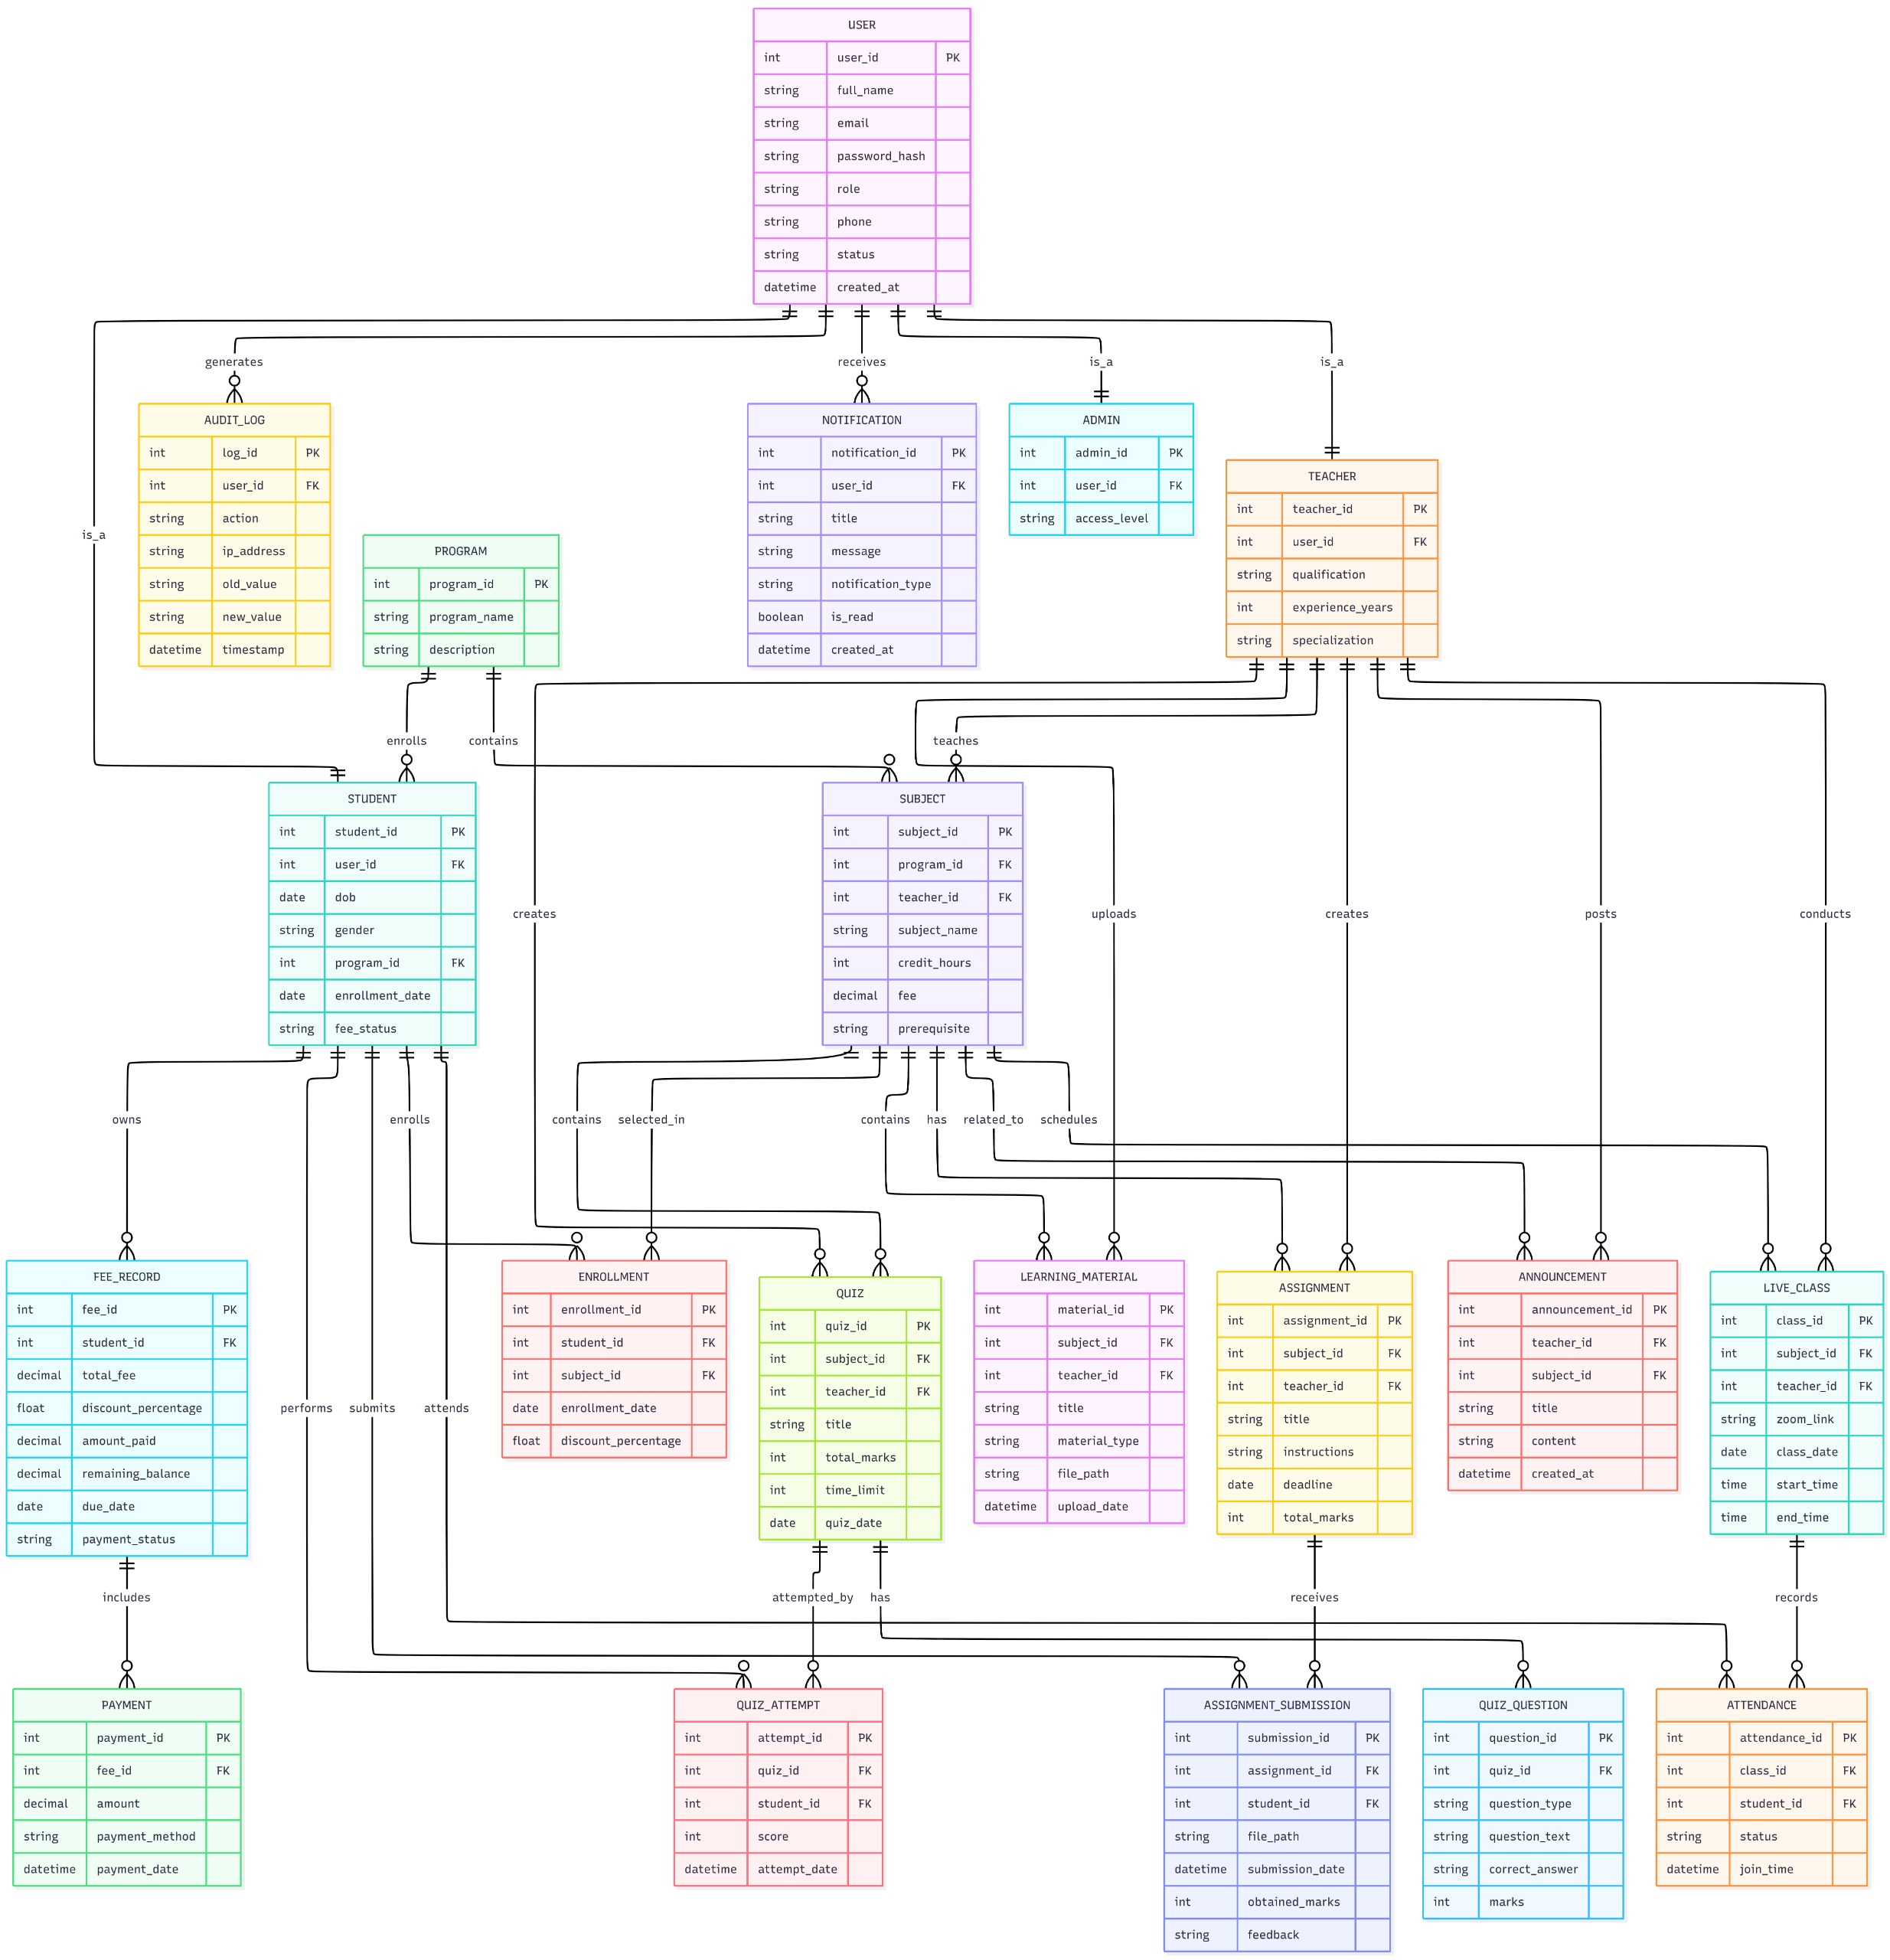
\includegraphics[width=1\linewidth]{erd.png}
            \label{fig:placeholder}
        \end{figure}
                
        \label{fig:placeholder}
    \end{figure}
        \caption{Entity Relationship Diagram --- AAK Academy Management System}
    \label{fig:erd}
\end{figure}

\subsection{ERD Design Decisions}

\begin{longtable}{|L{5cm}|L{9cm}|}
\hline
\textbf{Design Decision} & \textbf{Rationale} \\
\hline
\endfirsthead
\hline
\textbf{Design Decision} & \textbf{Rationale} \\
\hline
\endhead
Supertype/Subtype for users & Single USER table with role-specific tables (admin, teacher, student) avoids duplicate login credentials and simplifies authentication. \\
\hline
Separate enrollment table & Resolves the many-to-many relationship between students and subjects, allowing discount tracking per enrollment. \\
\hline
Separate payment table & One fee record can have multiple partial payments over time — normalizes the financial data. \\
\hline
Quiz questions as a separate entity & One quiz contains many questions; storing them in a child table supports normalization and flexible question management. \\
\hline
Attendance linked to live\_class & Attendance is recorded per scheduled class session, not per subject directly, enabling accurate session-level tracking. \\
\hline
Audit log as standalone entity & Tracks all system changes independently for security compliance, decoupled from business tables. \\
\hline
\end{longtable}

% ============================================================
%  CHAPTER 3: LOGICAL DATABASE DESIGN
% ============================================================
\chapter{LOGICAL DATABASE DESIGN}

\section{RELATIONAL SCHEMA}

\subsection{Module 1: User Management}

\textbf{user}(\underline{user\_id}, full\_name, email, password\_hash, role, phone, status, created\_at)
\begin{itemize}[noitemsep,topsep=2pt]
    \item PK: user\_id \quad | \quad UK: email
\end{itemize}

\textbf{admin}(\underline{admin\_id}, user\_id, access\_level)
\begin{itemize}[noitemsep,topsep=2pt]
    \item PK: admin\_id \quad | \quad FK: user\_id $\rightarrow$ user(user\_id) ON DELETE CASCADE \quad | \quad UK: user\_id
\end{itemize}

\textbf{teacher}(\underline{teacher\_id}, user\_id, qualification, experience\_years, specialization)
\begin{itemize}[noitemsep,topsep=2pt]
    \item PK: teacher\_id \quad | \quad FK: user\_id $\rightarrow$ user(user\_id) ON DELETE CASCADE \quad | \quad UK: user\_id
\end{itemize}

\textbf{student}(\underline{student\_id}, user\_id, dob, gender, program\_id, enrollment\_date, fee\_status)
\begin{itemize}[noitemsep,topsep=2pt]
    \item PK: student\_id \quad | \quad FK: user\_id $\rightarrow$ user(user\_id) ON DELETE CASCADE
    \item FK: program\_id $\rightarrow$ program(program\_id) ON DELETE SET NULL \quad | \quad UK: user\_id
\end{itemize}

\subsection{Module 2: Academic Structure}

\textbf{program}(\underline{program\_id}, program\_name, description)
\begin{itemize}[noitemsep,topsep=2pt]
    \item PK: program\_id
\end{itemize}

\textbf{subject}(\underline{subject\_id}, program\_id, teacher\_id, subject\_name, credit\_hours, fee, prerequisite)
\begin{itemize}[noitemsep,topsep=2pt]
    \item PK: subject\_id \quad | \quad FK: program\_id $\rightarrow$ program(program\_id) ON DELETE SET NULL
    \item FK: teacher\_id $\rightarrow$ teacher(teacher\_id) ON DELETE SET NULL
\end{itemize}

\textbf{enrollment}(\underline{enrollment\_id}, student\_id, subject\_id, enrollment\_date, discount\_percentage)
\begin{itemize}[noitemsep,topsep=2pt]
    \item PK: enrollment\_id \quad | \quad FK: student\_id $\rightarrow$ student(student\_id) ON DELETE CASCADE
    \item FK: subject\_id $\rightarrow$ subject(subject\_id) ON DELETE CASCADE
\end{itemize}

\subsection{Module 3: Finance}

\textbf{fee\_record}(\underline{fee\_id}, student\_id, total\_fee, discount\_percentage, amount\_paid, remaining\_balance, due\_date, payment\_status)
\begin{itemize}[noitemsep,topsep=2pt]
    \item PK: fee\_id \quad | \quad FK: student\_id $\rightarrow$ student(student\_id) ON DELETE CASCADE
\end{itemize}

\textbf{payment}(\underline{payment\_id}, fee\_id, amount, payment\_method, payment\_date)
\begin{itemize}[noitemsep,topsep=2pt]
    \item PK: payment\_id \quad | \quad FK: fee\_id $\rightarrow$ fee\_record(fee\_id) ON DELETE CASCADE
\end{itemize}

\subsection{Module 4: Learning \& Assessment}

\textbf{assignment}(\underline{assignment\_id}, subject\_id, teacher\_id, title, instructions, deadline, total\_marks)

\textbf{assignment\_submission}(\underline{submission\_id}, assignment\_id, student\_id, file\_path, submission\_date, obtained\_marks, feedback)

\textbf{quiz}(\underline{quiz\_id}, subject\_id, teacher\_id, title, total\_marks, time\_limit, quiz\_date)

\textbf{quiz\_question}(\underline{question\_id}, quiz\_id, question\_type, question\_text, correct\_answer, marks)
\begin{itemize}[noitemsep,topsep=2pt]
    \item FK: quiz\_id $\rightarrow$ quiz(quiz\_id) ON DELETE CASCADE
\end{itemize}

\textbf{quiz\_attempt}(\underline{attempt\_id}, quiz\_id, student\_id, score, attempt\_date)

\textbf{learning\_material}(\underline{material\_id}, subject\_id, teacher\_id, title, material\_type, file\_path, upload\_date)

\textbf{live\_class}(\underline{class\_id}, subject\_id, teacher\_id, zoom\_link, class\_date, start\_time, end\_time)

\textbf{attendance}(\underline{attendance\_id}, class\_id, student\_id, status, join\_time)
\begin{itemize}[noitemsep,topsep=2pt]
    \item FK: class\_id $\rightarrow$ live\_class(class\_id) ON DELETE CASCADE
    \item FK: student\_id $\rightarrow$ student(student\_id) ON DELETE CASCADE
\end{itemize}

\subsection{Module 5: Communication \& Security}

\textbf{announcement}(\underline{announcement\_id}, teacher\_id, subject\_id, title, content, created\_at)

\textbf{notification}(\underline{notification\_id}, user\_id, title, message, notification\_type, is\_read, created\_at)
\begin{itemize}[noitemsep,topsep=2pt]
    \item FK: user\_id $\rightarrow$ user(user\_id) ON DELETE CASCADE
\end{itemize}

\textbf{audit\_log}(\underline{log\_id}, user\_id, action, ip\_address, old\_value, new\_value, timestamp)
\begin{itemize}[noitemsep,topsep=2pt]
    \item FK: user\_id $\rightarrow$ user(user\_id) ON DELETE SET NULL
\end{itemize}

\subsection{Relationship Cardinality Summary}

\begin{longtable}{|L{5cm}|C{2.5cm}|L{5.5cm}|}
\hline
\textbf{Relationship} & \textbf{Type} & \textbf{Implementation} \\
\hline
\endfirsthead
\hline
\textbf{Relationship} & \textbf{Type} & \textbf{Implementation} \\
\hline
\endhead
user $\rightarrow$ admin / teacher / student & 1:0..1 & FK in subtype table with UNIQUE constraint \\
\hline
program $\rightarrow$ student & 1:N & program\_id FK in student \\
\hline
program $\rightarrow$ subject & 1:N & program\_id FK in subject \\
\hline
teacher $\rightarrow$ subject & 1:N & teacher\_id FK in subject \\
\hline
student $\leftrightarrow$ subject & M:N & enrollment junction table \\
\hline
student $\rightarrow$ fee\_record & 1:N & student\_id FK in fee\_record \\
\hline
fee\_record $\rightarrow$ payment & 1:N & fee\_id FK in payment \\
\hline
subject $\rightarrow$ assignment / quiz / material / live\_class & 1:N & subject\_id FK \\
\hline
assignment $\rightarrow$ submission & 1:N & assignment\_id FK \\
\hline
quiz $\rightarrow$ question / attempt & 1:N & quiz\_id FK \\
\hline
live\_class $\rightarrow$ attendance & 1:N & class\_id FK \\
\hline
\end{longtable}

\section{FUNCTIONAL DEPENDENCIES}

Key functional dependencies for the major tables are listed below using the notation A $\rightarrow$ B.

\textbf{USER:}
\begin{align*}
&\text{user\_id} \rightarrow \text{full\_name, email, password\_hash, role, phone, status, created\_at}\\
&\text{email} \rightarrow \text{user\_id, full\_name, role, status}
\end{align*}

\textbf{STUDENT:}
\begin{align*}
&\text{student\_id} \rightarrow \text{user\_id, dob, gender, program\_id, enrollment\_date, fee\_status}\\
&\text{user\_id} \rightarrow \text{student\_id}
\end{align*}

\textbf{SUBJECT:}
\begin{align*}
&\text{subject\_id} \rightarrow \text{program\_id, teacher\_id, subject\_name, credit\_hours, fee, prerequisite}
\end{align*}

\textbf{ENROLLMENT:}
\begin{align*}
&\text{enrollment\_id} \rightarrow \text{student\_id, subject\_id, enrollment\_date, discount\_percentage}\\
&\text{(student\_id, subject\_id)} \rightarrow \text{enrollment\_id}
\end{align*}

\textbf{FEE\_RECORD:}
\begin{align*}
&\text{fee\_id} \rightarrow \text{student\_id, total\_fee, discount\_percentage, amount\_paid, remaining\_balance, due\_date, payment\_status}
\end{align*}

\textbf{ATTENDANCE:}
\begin{align*}
&\text{attendance\_id} \rightarrow \text{class\_id, student\_id, status, join\_time}\\
&\text{(class\_id, student\_id)} \rightarrow \text{status, join\_time}
\end{align*}

\section{NORMALIZATION}

All tables in the AAMS schema satisfy \textbf{Third Normal Form (3NF)} and most satisfy \textbf{Boyce-Codd Normal Form (BCNF)}.

\subsection{First Normal Form (1NF)}

\textbf{Rule:} All attributes must be atomic — no repeating groups or multivalued attributes.

\begin{longtable}{|L{3cm}|C{2.5cm}|L{7cm}|}
\hline
\textbf{Table} & \textbf{1NF} & \textbf{Example} \\
\hline
\endfirsthead
\hline
\textbf{Table} & \textbf{1NF} & \textbf{Example} \\
\hline
\endhead
user & \checkmark & Each user has one email, one role — no comma-separated values \\
\hline
enrollment & \checkmark & One row per student-subject pair (M:N decomposed into junction table) \\
\hline
quiz\_question & \checkmark & Questions stored in separate rows, not as arrays within quiz \\
\hline
payment & \checkmark & Multiple payments stored as separate rows, not bundled in fee\_record \\
\hline
\end{longtable}

\textbf{Violation before 1NF (not used):}
\begin{lstlisting}[language=SQL]
student_enrollment(student_id, student_name, subjects_enrolled)
-- subjects_enrolled = "DB Systems, OOP, Data Structures"  [VIOLATION]
\end{lstlisting}

\textbf{After 1NF:}
\begin{lstlisting}[language=SQL]
enrollment(enrollment_id, student_id, subject_id, enrollment_date)  [CORRECT]
\end{lstlisting}

\subsection{Second Normal Form (2NF)}

\textbf{Rule:} Must be in 1NF; no partial dependencies on a composite primary key.

Since all tables use surrogate integer primary keys (auto-incremented), partial dependencies are inherently eliminated. No non-key attribute depends on only part of the key.

\textbf{Example — Partial dependency eliminated:}

Student name depends only on student\_id, not on the composite (student\_id, subject\_id) together. The name is stored in the USER table via student.user\_id, not duplicated in the enrollment table.

\subsection{Third Normal Form (3NF)}

\textbf{Rule:} Must be in 2NF; no transitive dependencies (non-key attribute determines another non-key attribute).

\begin{longtable}{|L{3cm}|L{5cm}|L{5cm}|}
\hline
\textbf{Table} & \textbf{Transitive Dependency Removed} & \textbf{How} \\
\hline
\endfirsthead
\hline
\textbf{Table} & \textbf{Transitive Dependency Removed} & \textbf{How} \\
\hline
\endhead
student & student $\rightarrow$ program\_name & program\_name stored in program table; only program\_id FK in student \\
\hline
subject & subject $\rightarrow$ teacher\_name & Teacher name in user table; only teacher\_id FK in subject \\
\hline
assignment & assignment $\rightarrow$ subject\_name, teacher\_name & Resolved via FK joins at query time \\
\hline
fee\_record & fee $\rightarrow$ student\_name & Student name retrieved via JOIN, not duplicated \\
\hline
\end{longtable}

\textbf{Example — Transitive dependency removed:}
\begin{lstlisting}[language=SQL]
-- BEFORE 3NF (violation):
subject(subject_id, subject_name, teacher_id, teacher_name, teacher_qualification)
-- teacher_name and teacher_qualification depend on teacher_id, not subject_id

-- AFTER 3NF (correct):
subject(subject_id, subject_name, teacher_id)
teacher(teacher_id, user_id, qualification, ...)
user(user_id, full_name, ...)
\end{lstlisting}

\subsection{Boyce-Codd Normal Form (BCNF)}

\textbf{Rule:} For every functional dependency X $\rightarrow$ Y, X must be a superkey.

\begin{longtable}{|L{3cm}|C{2.5cm}|L{7cm}|}
\hline
\textbf{Table} & \textbf{BCNF} & \textbf{Notes} \\
\hline
\endfirsthead
\hline
\textbf{Table} & \textbf{BCNF} & \textbf{Notes} \\
\hline
\endhead
user & \checkmark & email $\rightarrow$ all attributes; email is a candidate key \\
\hline
program & \checkmark & program\_id $\rightarrow$ all attributes \\
\hline
enrollment & \checkmark & enrollment\_id is PK; (student\_id, subject\_id) is also a candidate key \\
\hline
fee\_record & \checkmark & fee\_id $\rightarrow$ all attributes; no non-trivial FDs on non-superkeys \\
\hline
\end{longtable}

\subsection{Normalization Summary}

\begin{longtable}{|C{3cm}|C{2.5cm}|L{7cm}|}
\hline
\textbf{Normal Form} & \textbf{Status} & \textbf{Key Action Taken} \\
\hline
\endfirsthead
\hline
\textbf{Normal Form} & \textbf{Status} & \textbf{Key Action Taken} \\
\hline
\endhead
1NF & \checkmark Satisfied & Decomposed M:N enrollments; separated quiz questions into child table \\
\hline
2NF & \checkmark Satisfied & Used surrogate PKs; moved partial dependents to their parent tables \\
\hline
3NF & \checkmark Satisfied & Removed all transitive dependencies via FK references \\
\hline
BCNF & \checkmark Satisfied & All determinants are candidate or super keys in every table \\
\hline
\end{longtable}

% ============================================================
%  CHAPTER 4: IMPLEMENTATION
% ============================================================
\chapter{IMPLEMENTATION}

\section{LANGUAGE/FRAMEWORK}

The AAMS system is implemented using a \textbf{three-tier architecture}:

\begin{itemize}[noitemsep]
    \item \textbf{Frontend (Presentation Layer):} HTML5, CSS3, and vanilla JavaScript. A single-file application (\texttt{AAMS\_RoleBased.html}) delivers the entire role-based GUI. Chosen for portability — no build tools required.
    \item \textbf{Backend (Application Layer):} Node.js with Express.js (\texttt{server.js}). Provides RESTful API endpoints consumed by the frontend. Selected for its non-blocking I/O and seamless JSON handling.
    \item \textbf{Database (Data Layer):} MySQL 8.x (\texttt{aak\_academy} database). Chosen for its mature support of foreign key constraints, InnoDB transactions, stored procedures, and triggers.
    \item \textbf{Database Driver:} \texttt{mysql2} npm package with connection pooling (max 10 connections).
    \item \textbf{Configuration:} Environment variables managed via \texttt{dotenv} (\texttt{.env} file).
\end{itemize}

\subsection{DBMS Configuration}

\begin{longtable}{|L{4.5cm}|L{9cm}|}
\hline
\textbf{Parameter} & \textbf{Value} \\
\hline
\endfirsthead
\hline
\textbf{Parameter} & \textbf{Value} \\
\hline
\endhead
DBMS & MySQL 8.x \\
\hline
Database Name & aak\_academy \\
\hline
Database User & aak\_academy \\
\hline
Host & localhost \\
\hline
Port & 3306 (default) \\
\hline
Character Set & UTF-8 \\
\hline
Storage Engine & InnoDB (supports FK constraints and transactions) \\
\hline
\end{longtable}

\subsection{Constraints Implemented}

\begin{longtable}{|L{4cm}|C{2cm}|L{7.5cm}|}
\hline
\textbf{Constraint Type} & \textbf{Count} & \textbf{Examples} \\
\hline
\endfirsthead
\hline
\textbf{Constraint Type} & \textbf{Count} & \textbf{Examples} \\
\hline
\endhead
PRIMARY KEY & 20 & All 20 tables \\
\hline
FOREIGN KEY & 35+ & Cascading deletes on dependent records \\
\hline
UNIQUE & 4 & user.email, admin.user\_id, teacher.user\_id, student.user\_id \\
\hline
NOT NULL & 30+ & full\_name, email, role, and other critical fields \\
\hline
ENUM & 6 & role, status, gender, fee\_status, payment\_status, attendance.status \\
\hline
DEFAULT & 10+ & created\_at = CURRENT\_TIMESTAMP, status = 'active' \\
\hline
ON DELETE CASCADE & 20+ & Deleting a user removes their admin/teacher/student profile \\
\hline
ON DELETE SET NULL & 4 & program\_id, teacher\_id when the parent record is deleted \\
\hline
\end{longtable}

\subsection{Performance Indexes}

\begin{lstlisting}[language=SQL, caption={Indexes for query optimization}]
CREATE INDEX idx_user_email       ON user(email);
CREATE INDEX idx_student_program  ON student(program_id);
CREATE INDEX idx_subject_program  ON subject(program_id);
CREATE INDEX idx_subject_teacher  ON subject(teacher_id);
CREATE INDEX idx_enrollment_student ON enrollment(student_id);
CREATE INDEX idx_enrollment_subject ON enrollment(subject_id);
CREATE INDEX idx_fee_student      ON fee_record(student_id);
CREATE INDEX idx_payment_fee      ON payment(fee_id);
CREATE INDEX idx_attendance_class ON attendance(class_id);
CREATE INDEX idx_attendance_student ON attendance(student_id);
\end{lstlisting}

\section{DATABASE CONNECTIVITY}

The frontend HTML file communicates with the MySQL database through an Express REST API running on Node.js. The connection is managed via a \textbf{mysql2 connection pool} with a maximum of 10 simultaneous connections.

\subsection{Three-Tier Architecture Flow}

\begin{lstlisting}[language=SQL, caption={Connection pool configuration (server.js)}]
const pool = mysql.createPool({
  host:     process.env.DB_HOST,
  user:     process.env.DB_USER,
  password: process.env.DB_PASSWORD,
  database: process.env.DB_NAME,
  waitForConnections: true,
  connectionLimit: 10,
  dateStrings: true,
});
\end{lstlisting}

\subsection{REST API Endpoints}

\begin{longtable}{|L{4.5cm}|L{4.5cm}|L{5cm}|}
\hline
\textbf{Method} & \textbf{Endpoint} & \textbf{Description} \\
\hline
\endfirsthead
\hline
\textbf{Method} & \textbf{Endpoint} & \textbf{Description} \\
\hline
\endhead
GET & /api/health & Database connectivity check \\
\hline
POST & /api/login & User authentication (email + role) \\
\hline
GET & /api/data & Bulk load all data for dashboard \\
\hline
GET & /api/dashboard/stats & Admin dashboard live statistics \\
\hline
GET/POST/PUT/DELETE & /api/students & Student CRUD operations \\
\hline
GET/POST/PUT/DELETE & /api/teachers & Teacher CRUD operations \\
\hline
GET/POST/PUT/DELETE & /api/programs & Programme CRUD operations \\
\hline
GET/POST/PUT/DELETE & /api/subjects & Subject CRUD operations \\
\hline
GET/POST/PUT/DELETE & /api/enrollment & Enrollment CRUD operations \\
\hline
GET/POST/PUT/DELETE & /api/assignments & Assignment CRUD operations \\
\hline
GET/POST/PUT/DELETE & /api/quizzes & Quiz CRUD operations \\
\hline
GET/POST/PUT/DELETE & /api/liveclasses & Live class CRUD operations \\
\hline
GET/POST/PUT/DELETE & /api/attendance & Attendance CRUD operations \\
\hline
GET/POST/PUT/DELETE & /api/fees & Fee record CRUD operations \\
\hline
GET/POST/PUT/DELETE & /api/materials & Learning material CRUD \\
\hline
GET/POST/PUT/DELETE & /api/announcements & Announcement CRUD \\
\hline
GET/POST/PUT/DELETE & /api/users & User CRUD operations \\
\hline
GET & /api/notifications & Notifications list \\
\hline
GET & /api/auditlog & Audit log entries (read-only) \\
\hline
\end{longtable}

\subsection{Security Measures}

\begin{longtable}{|L{4cm}|L{9.5cm}|}
\hline
\textbf{Measure} & \textbf{Implementation} \\
\hline
\endfirsthead
\hline
\textbf{Measure} & \textbf{Implementation} \\
\hline
\endhead
Parameterized queries & All SQL uses \texttt{?} placeholders — prevents SQL injection attacks \\
\hline
Role-based login & Email + role combination validated against database on every login \\
\hline
FK constraints & Prevents orphaned records from being created \\
\hline
Cascade deletes & Automatic cleanup of all dependent child records \\
\hline
Audit logging & All significant operations recorded in audit\_log table \\
\hline
\end{longtable}

\section{STORED PROCEDURES AND FUNCTIONS}

\begin{longtable}{|C{0.5cm}|L{3.5cm}|C{2cm}|L{3.5cm}|L{2.5cm}|L{2cm}|}
\hline
\textbf{\#} & \textbf{Object Name} & \textbf{Type} & \textbf{Description} & \textbf{Input Parameters} & \textbf{Output} \\
\hline
\endfirsthead
\hline
\textbf{\#} & \textbf{Object Name} & \textbf{Type} & \textbf{Description} & \textbf{Input Parameters} & \textbf{Output} \\
\hline
\endhead
1 & sp\_CreateStudent & Stored Procedure & Creates a new user and student record atomically; logs the action in audit\_log & p\_name, p\_email, p\_phone, p\_status, p\_dob, p\_gender, p\_program\_name, p\_enrolled\_date & None (INSERT) \\
\hline
2 & sp\_UpdateStudent & Stored Procedure & Updates an existing student's profile in both user and student tables; logs the update & p\_student\_id, p\_name, p\_status, p\_dob, p\_gender, p\_program\_name, p\_enrolled\_date & None (UPDATE) \\
\hline
3 & sp\_DeleteStudent & Stored Procedure & Deletes a student's user record, cascading to all child records; logs the deletion & p\_student\_id & None (DELETE) \\
\hline
4 & trg\_AutoGenerateFeeRecord & Trigger (AFTER INSERT on enrollment) & Automatically creates a fee\_record when a student enrolls in a subject, computing the discounted balance & NEW.student\_id, NEW.subject\_id, NEW.discount\_percentage & Inserts into fee\_record \\
\hline
\end{longtable}

\subsection{Stored Procedure: sp\_CreateStudent}

\begin{lstlisting}[language=SQL, caption={Stored procedure for creating a student}]
CREATE PROCEDURE sp_CreateStudent(
    IN p_name VARCHAR(100),
    IN p_email VARCHAR(100),
    IN p_phone VARCHAR(20),
    IN p_status VARCHAR(20),
    IN p_dob DATE,
    IN p_gender VARCHAR(20),
    IN p_program_name VARCHAR(100),
    IN p_enrolled_date DATE
)
BEGIN
    DECLARE v_user_id INT;
    DECLARE v_program_id INT;

    SELECT program_id INTO v_program_id
    FROM program WHERE LOWER(program_name) = LOWER(p_program_name) LIMIT 1;

    INSERT INTO user (full_name, email, password_hash, role, phone, status)
    VALUES (p_name, LOWER(p_email), 'default_hash', 'student', p_phone, LOWER(p_status));

    SET v_user_id = LAST_INSERT_ID();

    INSERT INTO student (user_id, dob, gender, program_id, enrollment_date, fee_status)
    VALUES (v_user_id, p_dob, LOWER(p_gender), v_program_id, p_enrolled_date, 'unpaid');

    INSERT INTO audit_log (user_id, action, old_value, new_value)
    VALUES (1, 'INSERT student', NULL,
            CONCAT('Student ', p_name, ' registered via sp_CreateStudent'));
END;
\end{lstlisting}

\subsection{Trigger: trg\_AutoGenerateFeeRecord}

\begin{lstlisting}[language=SQL, caption={Trigger for automatic fee record generation on enrollment}]
CREATE TRIGGER trg_AutoGenerateFeeRecord
AFTER INSERT ON enrollment
FOR EACH ROW
BEGIN
    DECLARE v_subject_fee DECIMAL(10,2);
    DECLARE v_final_fee   DECIMAL(10,2);

    SELECT fee INTO v_subject_fee
    FROM subject WHERE subject_id = NEW.subject_id;

    SET v_final_fee = v_subject_fee
                    - (v_subject_fee * (NEW.discount_percentage / 100));

    INSERT INTO fee_record
        (student_id, total_fee, discount_percentage, amount_paid,
         remaining_balance, due_date, payment_status)
    VALUES
        (NEW.student_id, v_subject_fee, NEW.discount_percentage, 0.00,
         v_final_fee, DATE_ADD(CURDATE(), INTERVAL 30 DAY), 'unpaid');
END;
\end{lstlisting}

\subsection{Key SQL Queries}

\begin{lstlisting}[language=SQL, caption={Login authentication query}]
SELECT u.user_id, u.full_name, u.email, u.role, u.status,
       a.admin_id, t.teacher_id, s.student_id
FROM user u
LEFT JOIN admin   a ON u.user_id = a.user_id
LEFT JOIN teacher t ON u.user_id = t.user_id
LEFT JOIN student s ON u.user_id = s.user_id
WHERE u.email = ? AND u.role = ? AND u.status = 'active';
\end{lstlisting}

\begin{lstlisting}[language=SQL, caption={Student list with programme using JOIN}]
SELECT s.student_id, u.full_name, p.program_name, s.dob, s.enrollment_date
FROM student s
JOIN user u ON s.user_id = u.user_id
LEFT JOIN program p ON s.program_id = p.program_id;
\end{lstlisting}

\begin{lstlisting}[language=SQL, caption={Dashboard revenue aggregation}]
SELECT COALESCE(SUM(amount_paid), 0) AS total FROM fee_record;
\end{lstlisting}

\begin{lstlisting}[language=SQL, caption={Attendance rate calculation}]
SELECT ROUND(
    SUM(CASE WHEN status='present' THEN 1 ELSE 0 END) * 100.0 / COUNT(*), 1
) AS attendance_rate
FROM attendance;
\end{lstlisting}

\section{INTERFACES}

\subsection{GUI Design Philosophy}

The GUI follows a \textbf{modern, clean, role-based dashboard} design with a consistent green/gold colour scheme representing AAK Academy branding, fixed sidebar navigation, card-based dashboards, modal dialogs for CRUD forms, and toast notifications for user feedback.

\subsection{Colour Palette}

\begin{longtable}{|L{3.5cm}|C{2.5cm}|L{8cm}|}
\hline
\textbf{Variable} & \textbf{Hex} & \textbf{Usage} \\
\hline
\endfirsthead
\hline
\textbf{Variable} & \textbf{Hex} & \textbf{Usage} \\
\hline
\endhead
--green-deep & \#1a4731 & Sidebar, headers, primary buttons \\
\hline
--green-mid & \#2d7a4f & Hover states and accents \\
\hline
--gold & \#c9a227 & Admin badges and highlights \\
\hline
--surface & \#ffffff & Cards and modals \\
\hline
--danger & \#c0392b & Delete buttons and errors \\
\hline
--success & \#27ae60 & Paid status tags and present attendance \\
\hline
\end{longtable}

\subsection{Role-Based Navigation}

\textbf{Admin} (17 pages): Dashboard, Students, Teachers, Programs, Subjects, Enrollment, Assignments, Quizzes, Live Classes, Attendance, Materials, Fees, Announcements, Notifications, Users, Audit Log.

\textbf{Teacher} (8 pages): Dashboard, My Subjects, Assignments, Quizzes, Live Classes, Mark Attendance, Materials, Announcements.

\textbf{Student} (9 pages): Dashboard, My Subjects, My Attendance, Assignments, Quizzes, Live Classes, Materials, My Fees, Announcements.

\subsection{Sample Data Statistics}

\begin{longtable}{|L{5cm}|C{3.5cm}|}
\hline
\textbf{Table} & \textbf{Records} \\
\hline
\endfirsthead
\hline
\textbf{Table} & \textbf{Records} \\
\hline
\endhead
user & 49 \\ \hline
admin & 2 \\ \hline
teacher & 23 \\ \hline
student & 24 \\ \hline
program & 24 \\ \hline
subject & 20 \\ \hline
enrollment & 28 \\ \hline
fee\_record & 24 \\ \hline
payment & 21 \\ \hline
assignment & 22 \\ \hline
assignment\_submission & 21 \\ \hline
quiz & 22 \\ \hline
quiz\_question & 21 \\ \hline
quiz\_attempt & 21 \\ \hline
learning\_material & 21 \\ \hline
announcement & 22 \\ \hline
live\_class & 22 \\ \hline
attendance & 22 \\ \hline
notification & 20 \\ \hline
audit\_log & 20 \\ \hline
\textbf{Total} & \textbf{400+} \\
\hline
\end{longtable}

% ============================================================
% SCREENSHOTS
% ============================================================

\subsection{Screenshots}

\textit{Instructions: Run \texttt{npm start}, open \texttt{http://localhost:3000}, and capture the following system interfaces.}

% ============================================================
% LOGIN SCREEN
% ============================================================

\subsubsection*{Login Screen}

\begin{figure}[H]
\centering
\includegraphics[width=\textwidth]{}
\begin{figure}
    \centering
    \includegraphics[width=1\linewidth]{}
\begin{figure}
        \centering
        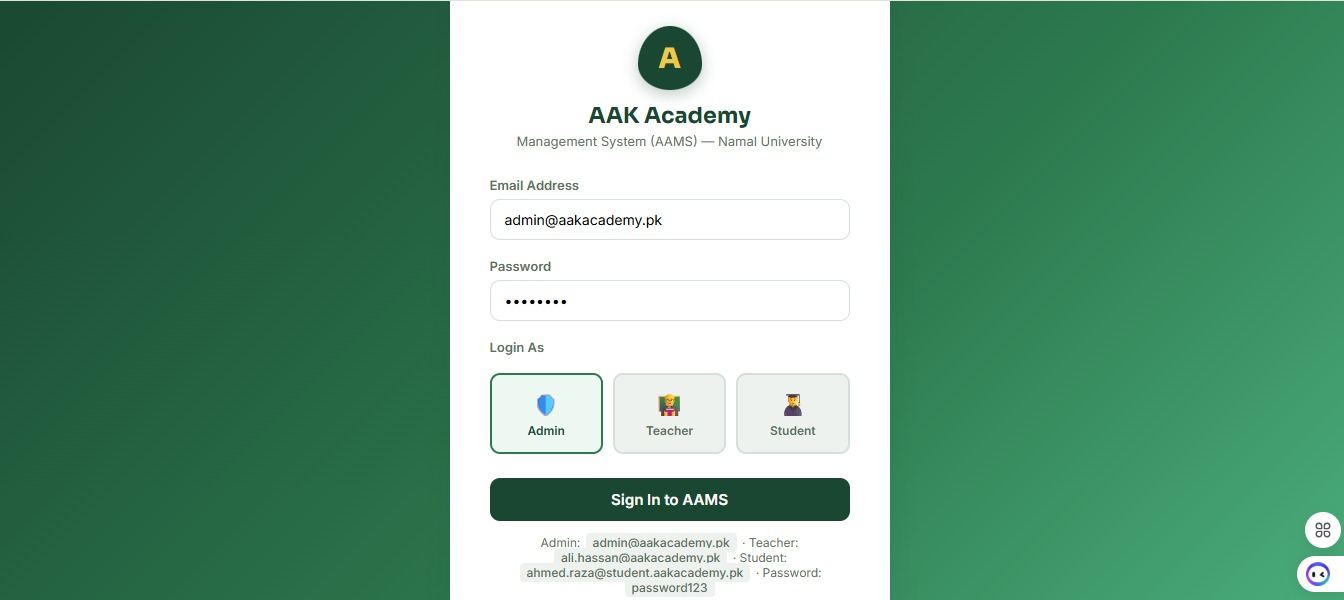
\includegraphics[width=1\linewidth]{mainlogin.png}
      
        \label{fig:placeholder}
    \end{figure}
        \label{fig:placeholder}
\end{figure}
\caption{Main Login Screen}
\end{figure}

% ============================================================
% ADMIN MODULE
% ============================================================

\subsubsection*{Admin Module}

\begin{figure}[H]
\centering
\includegraphics[width=\textwidth]{}
\begin{figure}
    \centering
    \includegraphics[width=0.8\linewidth]{}
\begin{figure}
    \centering
    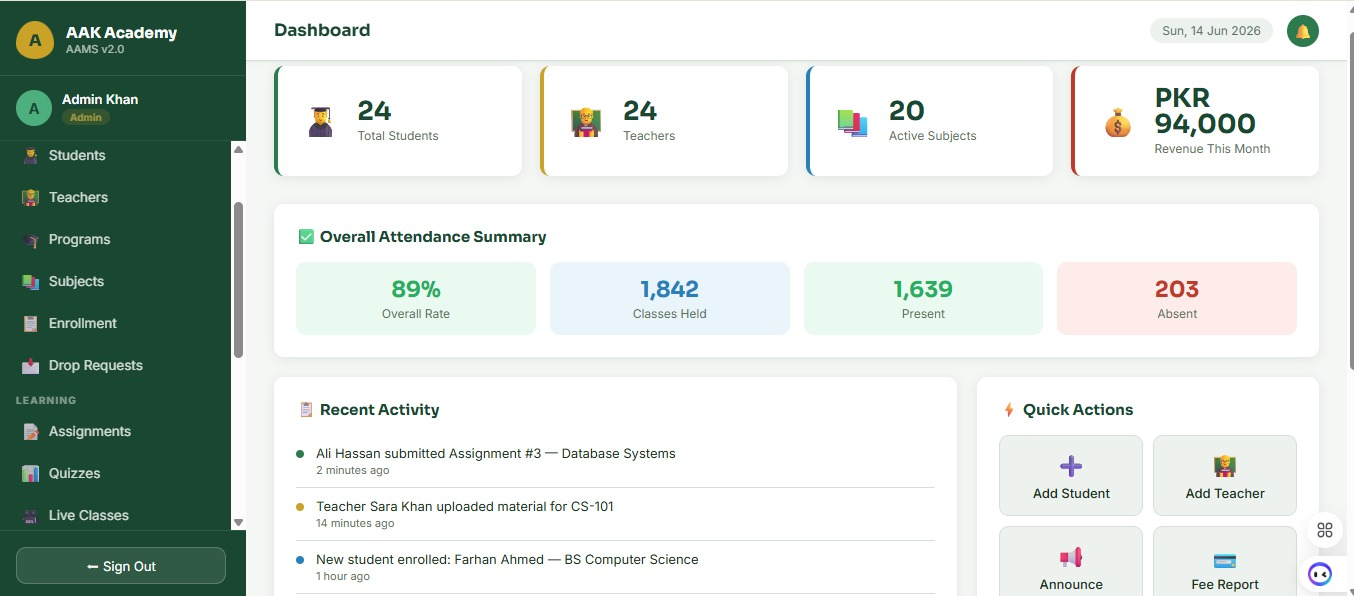
\includegraphics[width=0.8\linewidth]{admin main dashboard.png}

    \label{fig:placeholder}
\end{figure}
    \label{fig:placeholder}
\end{figure}
\caption{Admin Main Dashboard}
\end{figure}

\begin{figure}[H]
\centering
\includegraphics[width=\textwidth]{}
\begin{figure}
    \centering
    \includegraphics[width=0.8\linewidth]{}
\begin{figure}
        \centering
        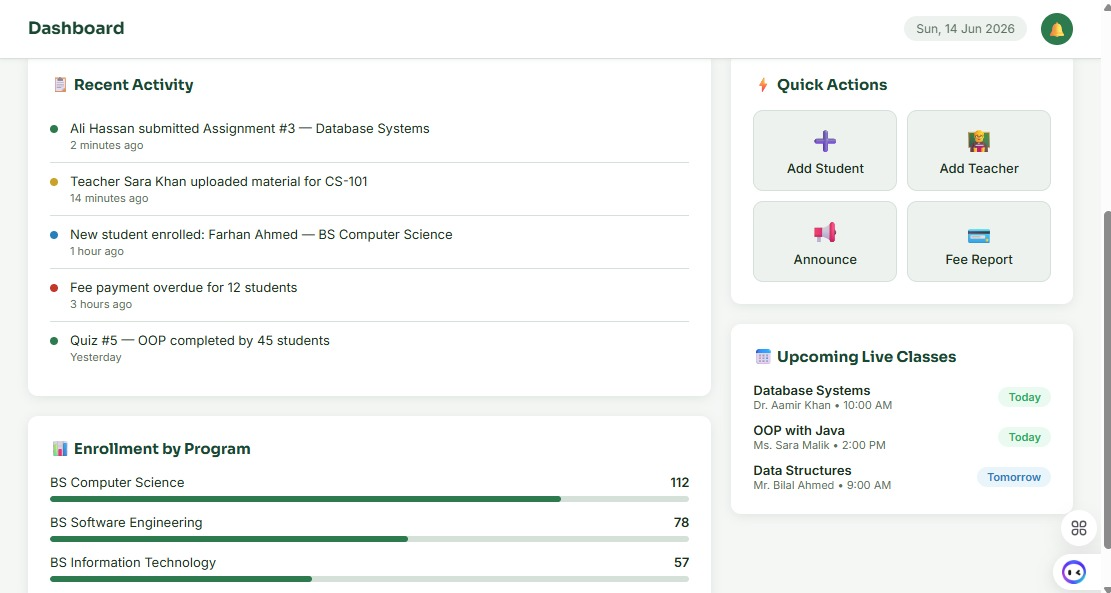
\includegraphics[width=0.8\linewidth]{quickactionsadmin.png}
        \label{fig:placeholder}
    \end{figure}
        \label{fig:placeholder}
\end{figure}
\caption{Admin Quick Actions and Recent Activity}
\end{figure}

\begin{figure}[H]
\centering
\includegraphics[width=\textwidth]{}
\begin{figure}
    \centering
    \includegraphics[width=0.8\linewidth]{}
\begin{figure}
        \centering
        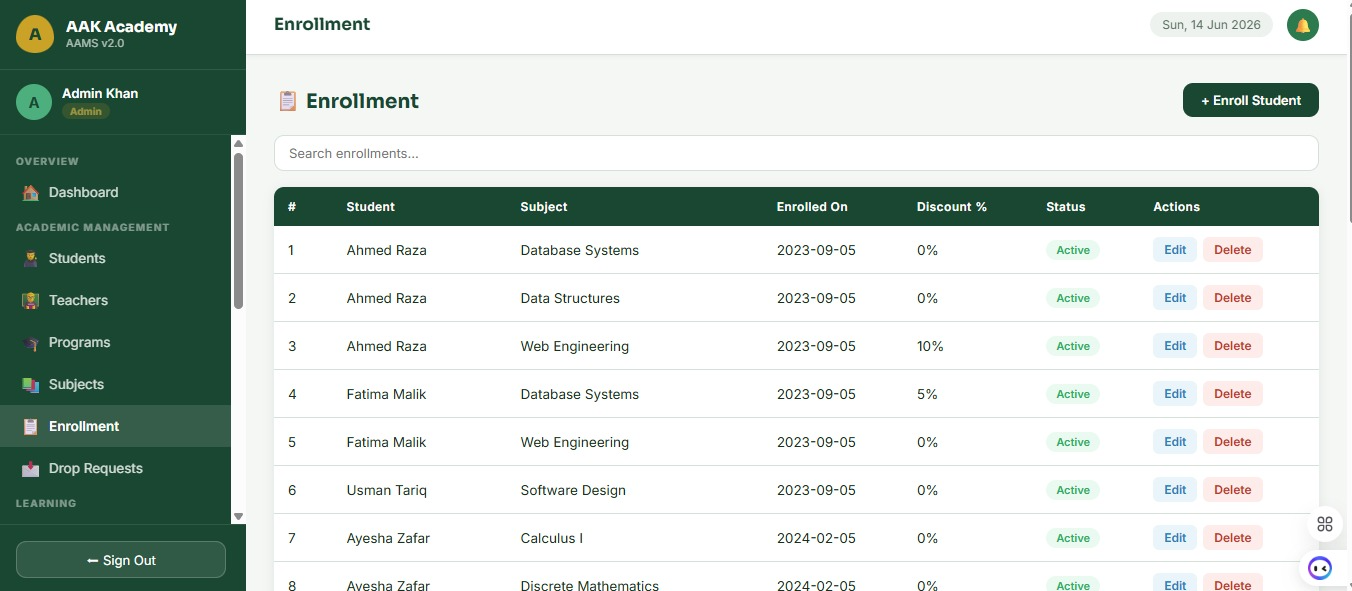
\includegraphics[width=0.8\linewidth]{enrollment.png}
        \label{fig:placeholder}
    \end{figure}
        \label{fig:placeholder}
\end{figure}
\caption{Student Enrollment (Admin Only)}
\end{figure}

\begin{figure}[H]
\centering
\includegraphics[width=\textwidth]{}
\begin{figure}
    \centering
    \includegraphics[width=0.8\linewidth]{}
\begin{figure}
        \centering
        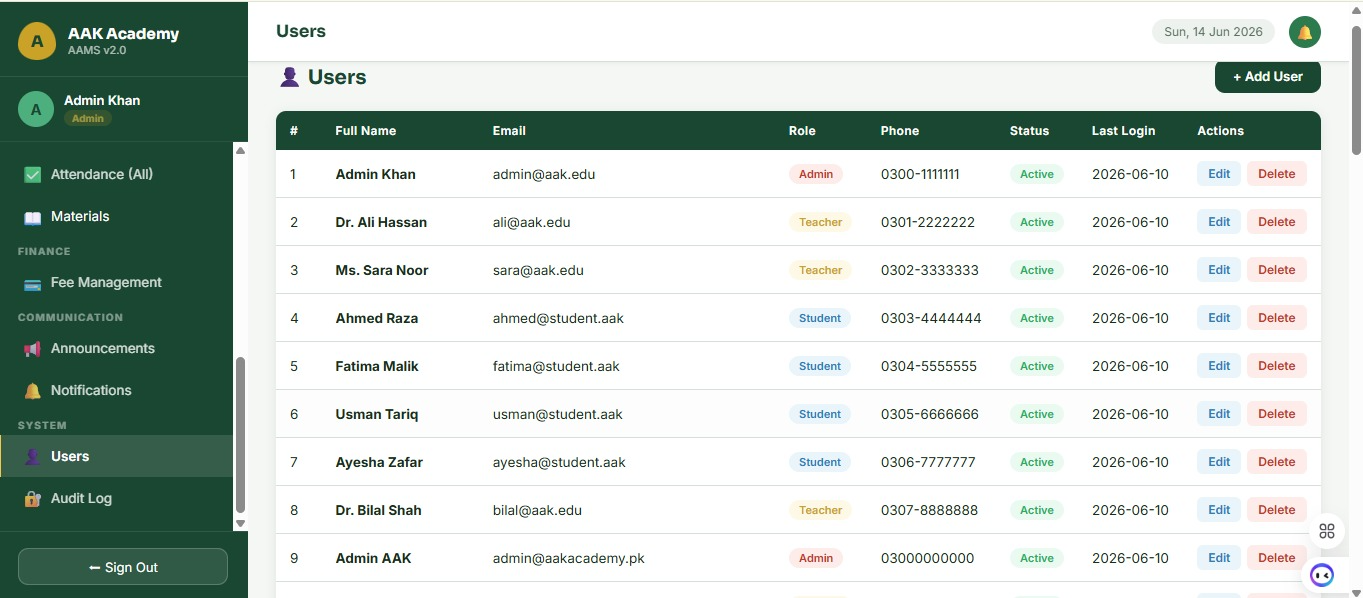
\includegraphics[width=0.8\linewidth]{usermanagement.png}
        \label{fig:placeholder}
    \end{figure}
        \label{fig:placeholder}
\end{figure}
\caption{User Management (Admin Only)}
\end{figure}

\begin{figure}[H]
\centering
\includegraphics[width=\textwidth]{}
\begin{figure}
    \centering
    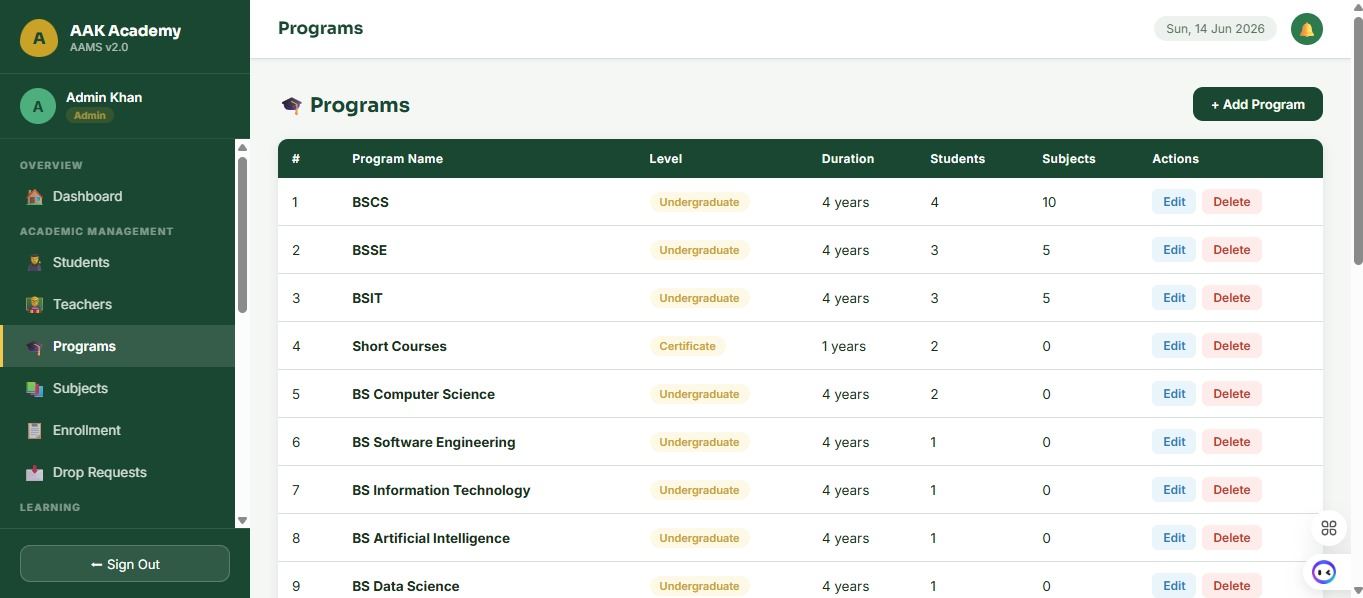
\includegraphics[width=0.8\linewidth]{programmanagement.png}
    \label{fig:placeholder}
\end{figure}
\caption{Program Management (Admin Only)}
\end{figure}

\begin{figure}[H]
\centering
\includegraphics[width=\textwidth]{}
\begin{figure}
    \centering
    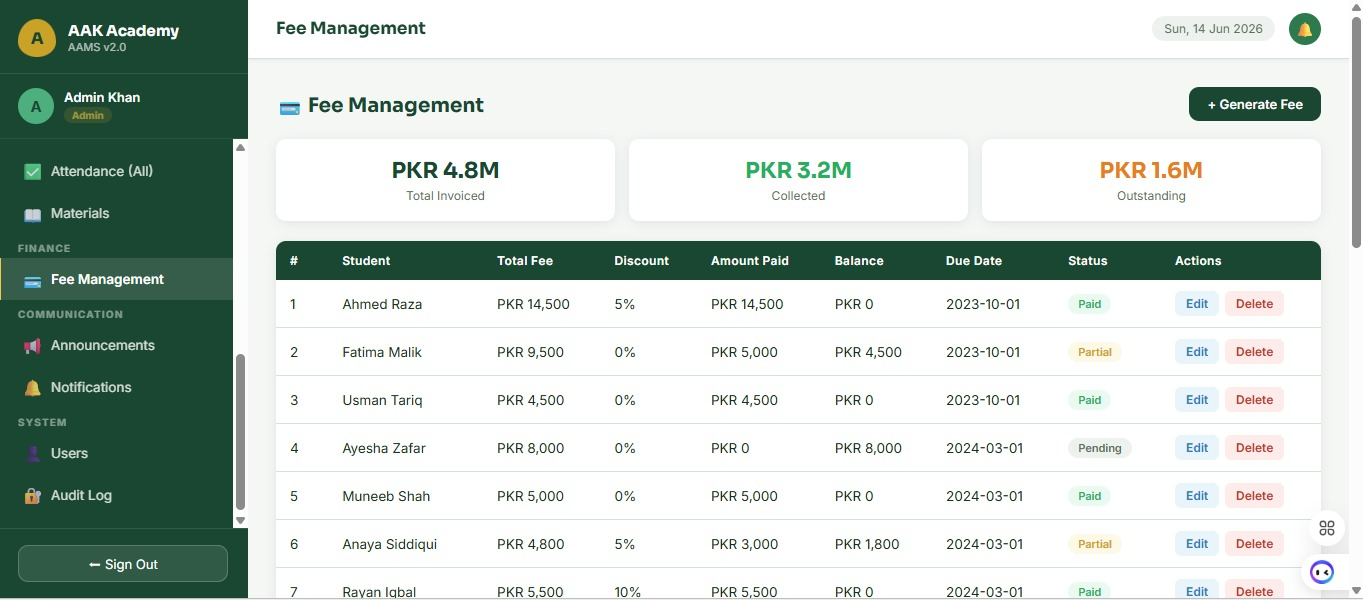
\includegraphics[width=0.8\linewidth]{feemanagement.png}
    \label{fig:placeholder}
\end{figure}
\caption{Fee Management (Admin Only)}
\end{figure}

\begin{figure}[H]
\centering
\includegraphics[width=\textwidth]{}
\begin{figure}
    \centering
    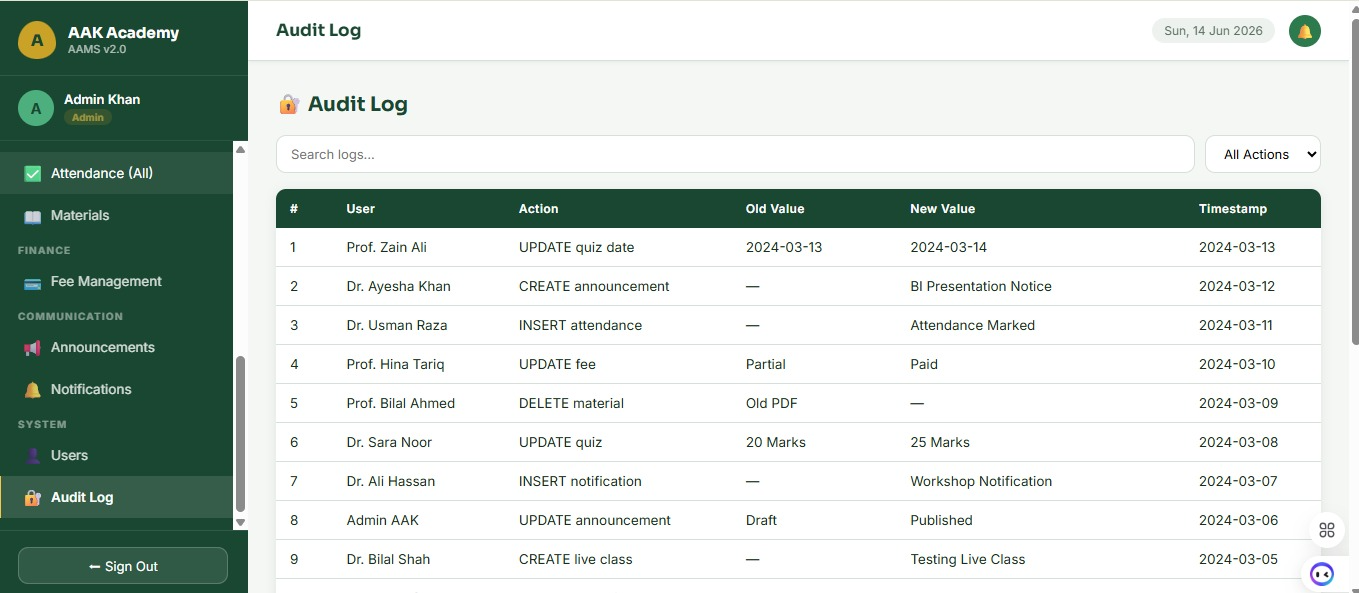
\includegraphics[width=0.8\linewidth]{auditlog.png}
    
    \label{fig:placeholder}
\end{figure}
\caption{Audit Log (Admin Only)}
\end{figure}

\begin{figure}[H]
\centering
\includegraphics[width=\textwidth]{}
\begin{figure}
    \centering
    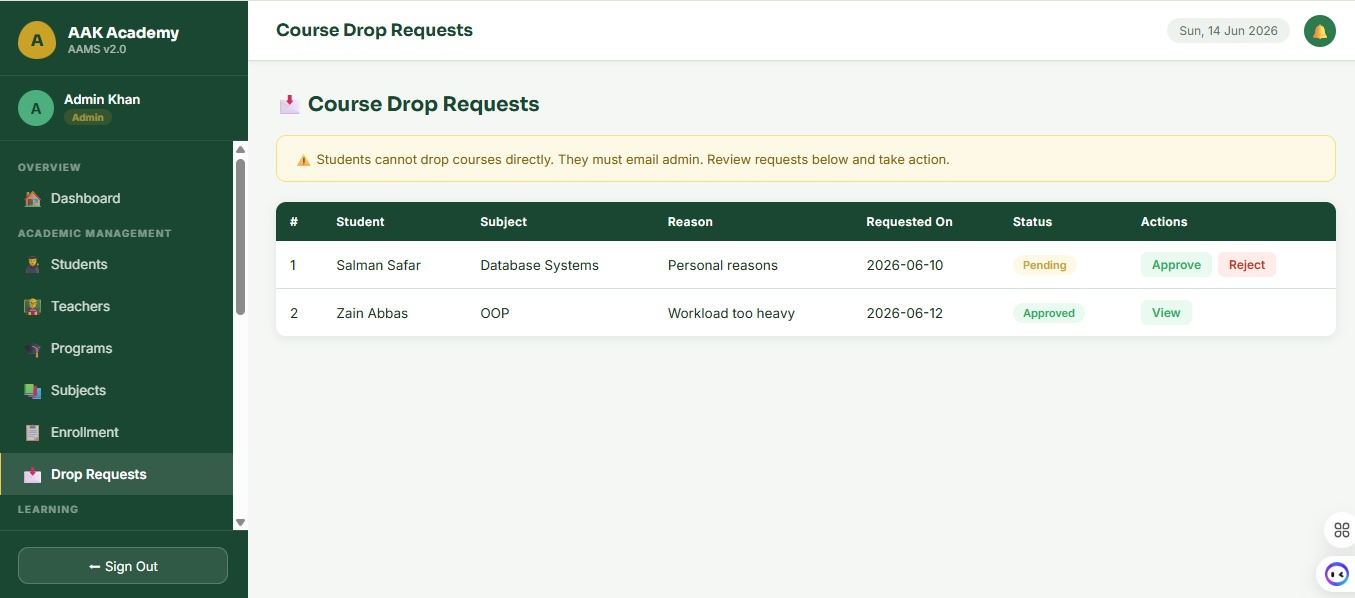
\includegraphics[width=0.8\linewidth]{courrsedropreq.png}
    \label{fig:placeholder}
\end{figure}
\caption{Student Course Drop Requests (Admin Only)}
\end{figure}

\begin{figure}[H]
\centering
\includegraphics[width=\textwidth]{}
\begin{figure}
    \centering
    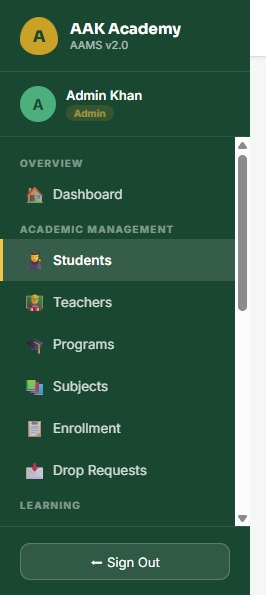
\includegraphics[width=0.3\linewidth]{adminmainfunc.png}
    \label{fig:placeholder}
\end{figure}
\caption{Admin Main Functionalities}
\end{figure}

\clearpage

% ============================================================
% TEACHER MODULE
% ============================================================

\subsubsection*{Teacher Module}

\begin{figure}[H]
\centering
\includegraphics[width=\textwidth]{}
\begin{figure}
    \centering
    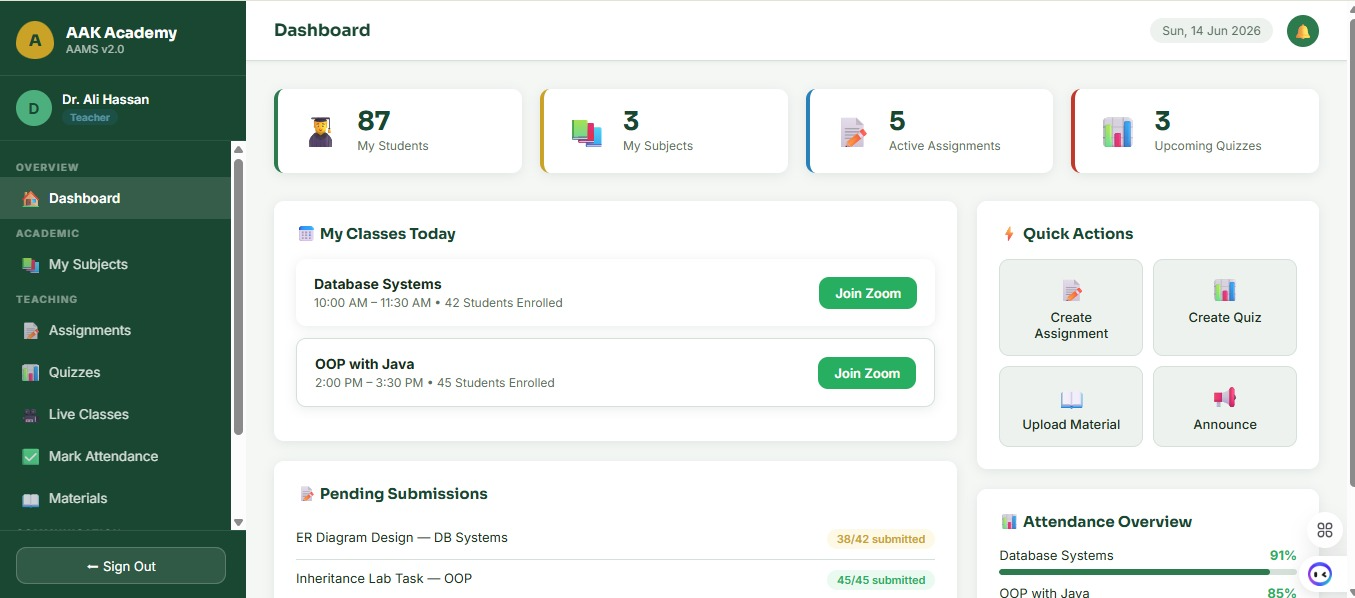
\includegraphics[width=0.8\linewidth]{teachermaindashboard.png}
    \label{fig:placeholder}
\end{figure}
\caption{Teacher Main Dashboard}
\end{figure}

\begin{figure}[H]
\centering
\includegraphics[width=\textwidth]{}
\begin{figure}
    \centering
    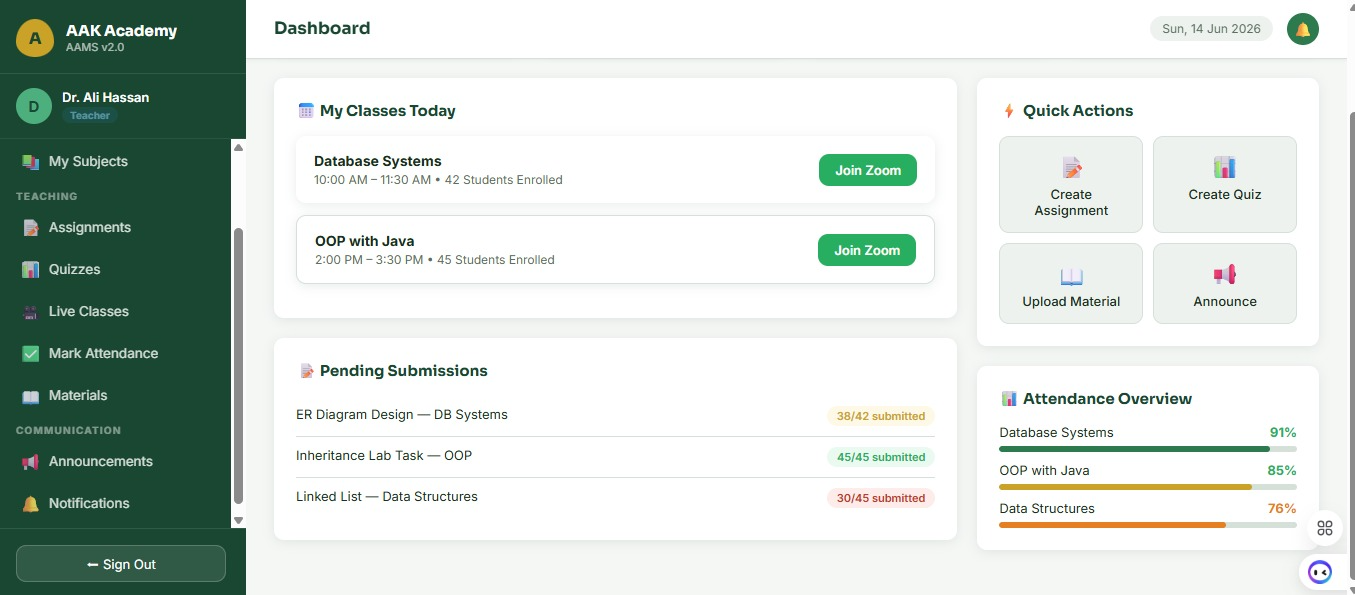
\includegraphics[width=0.8\linewidth]{teacherquickaction.png}
    \label{fig:placeholder}
\end{figure}
\caption{Teacher Quick Action Panel}
\end{figure}

\begin{figure}[H]
\centering
\includegraphics[width=\textwidth]{}
\begin{figure}
    \centering
    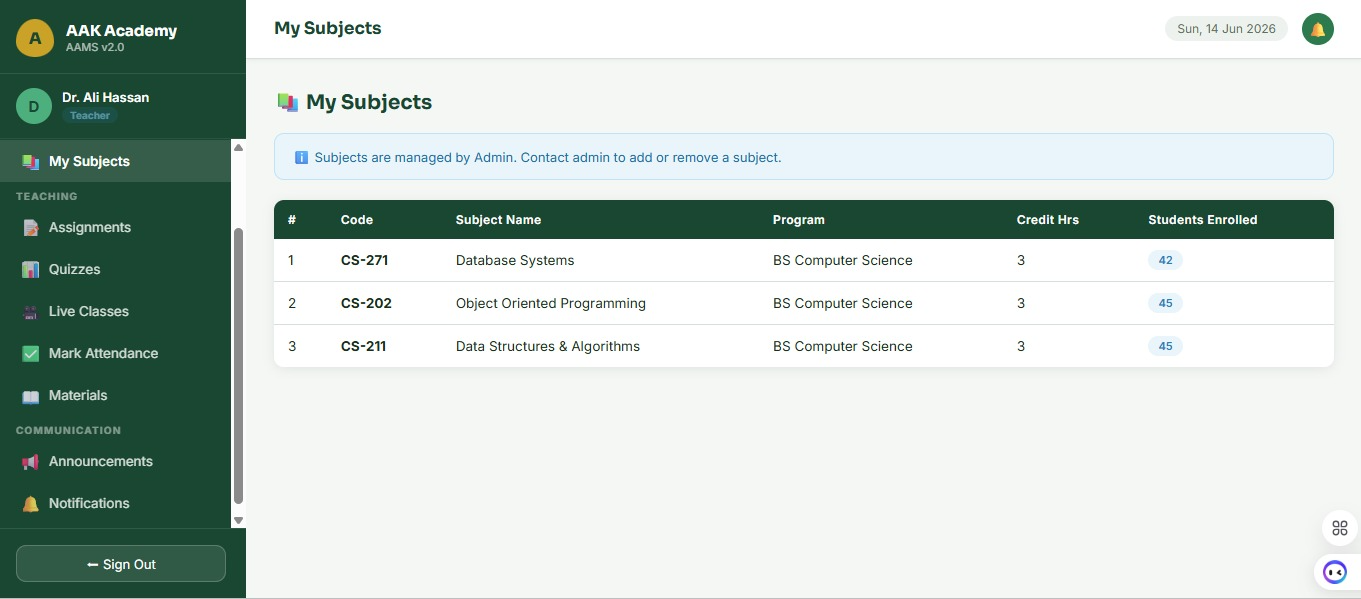
\includegraphics[width=0.8\linewidth]{teachersubjects.png}
    \label{fig:placeholder}
\end{figure}
\caption{Teacher Subjects}
\end{figure}

\begin{figure}[H]
\centering
\includegraphics[width=\textwidth]{}
\begin{figure}
    \centering
    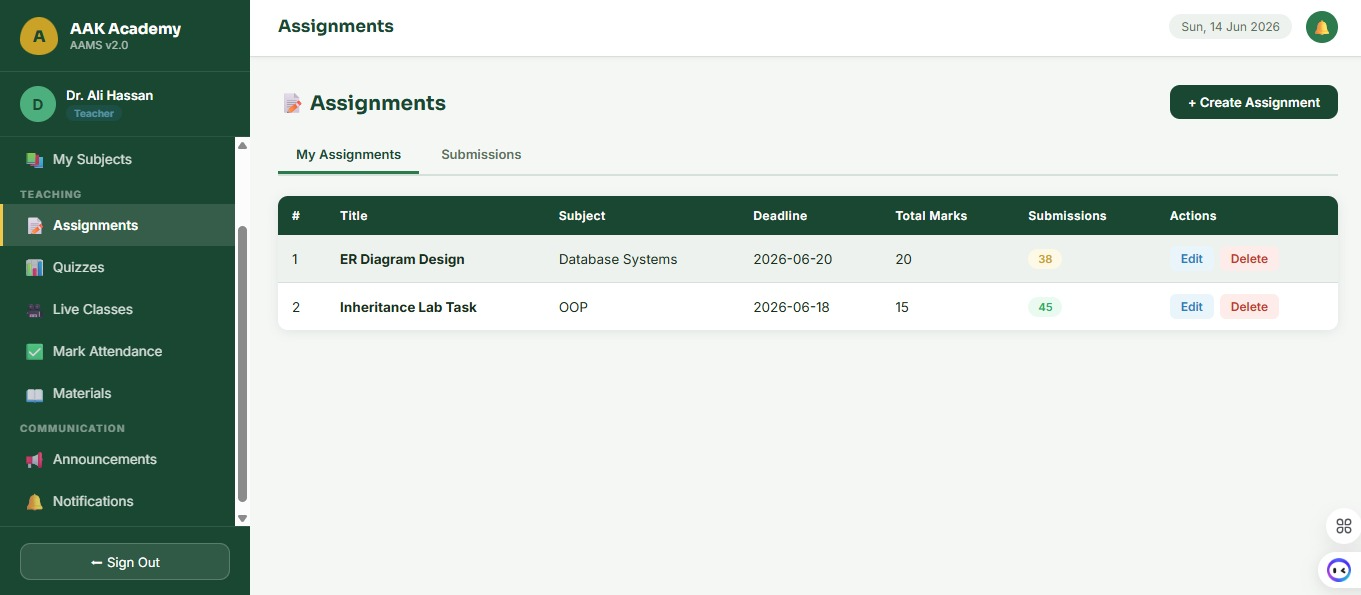
\includegraphics[width=0.8\linewidth]{teacherassignment.png}
  
    \label{fig:placeholder}
\end{figure}
\caption{Teacher Assignment Section}
\end{figure}

\begin{figure}[H]
\centering
\includegraphics[width=\textwidth]{}
\begin{figure}
    \centering
    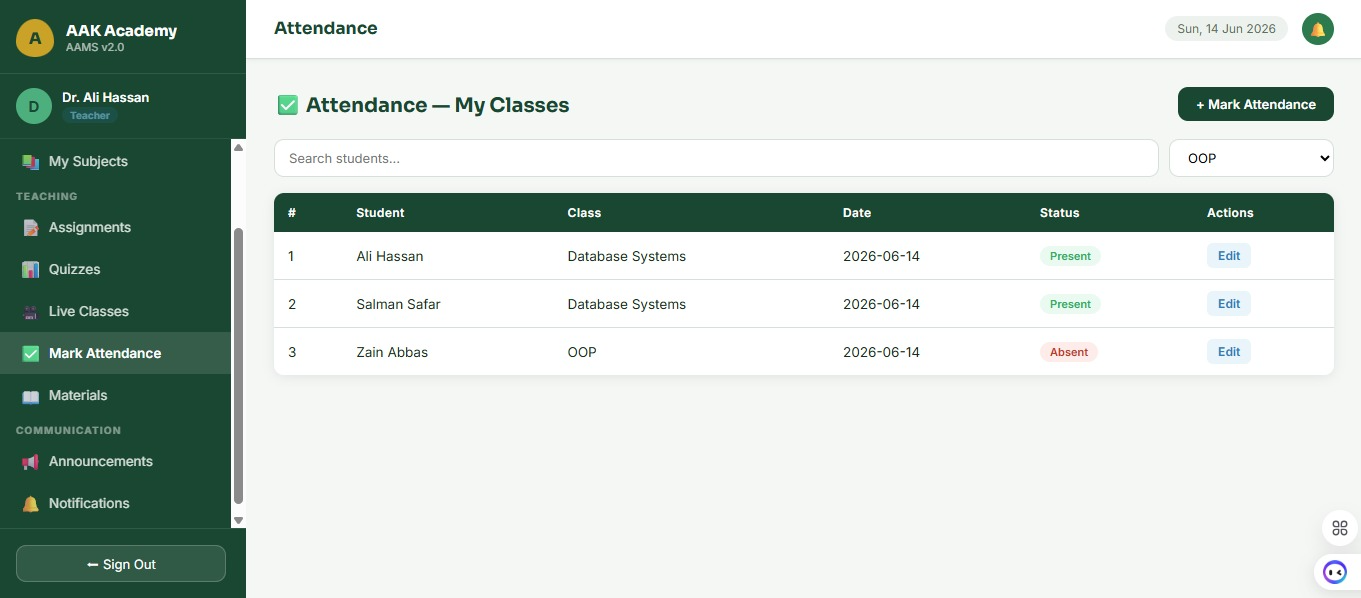
\includegraphics[width=0.8\linewidth]{teacherattendence.png}
   
    \label{fig:placeholder}
\end{figure}
\caption{Teacher Attendance Marking}
\end{figure}

\begin{figure}[H]
\centering
\includegraphics[width=\textwidth]{}
\begin{figure}
    \centering
    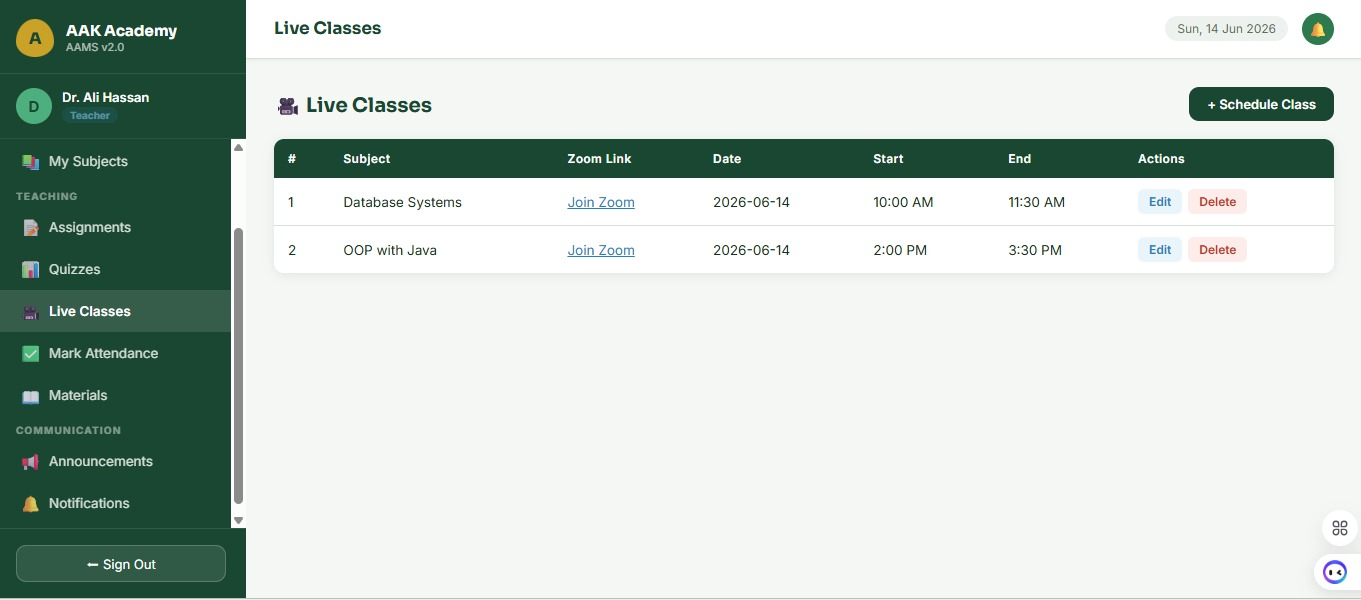
\includegraphics[width=0.8\linewidth]{teacherliveclass.png}
    \label{fig:placeholder}
\end{figure}
\caption{Teacher Live Class Integration}
\end{figure}

\begin{figure}[H]
\centering
\includegraphics[width=\textwidth]{}
\begin{figure}
    \centering
    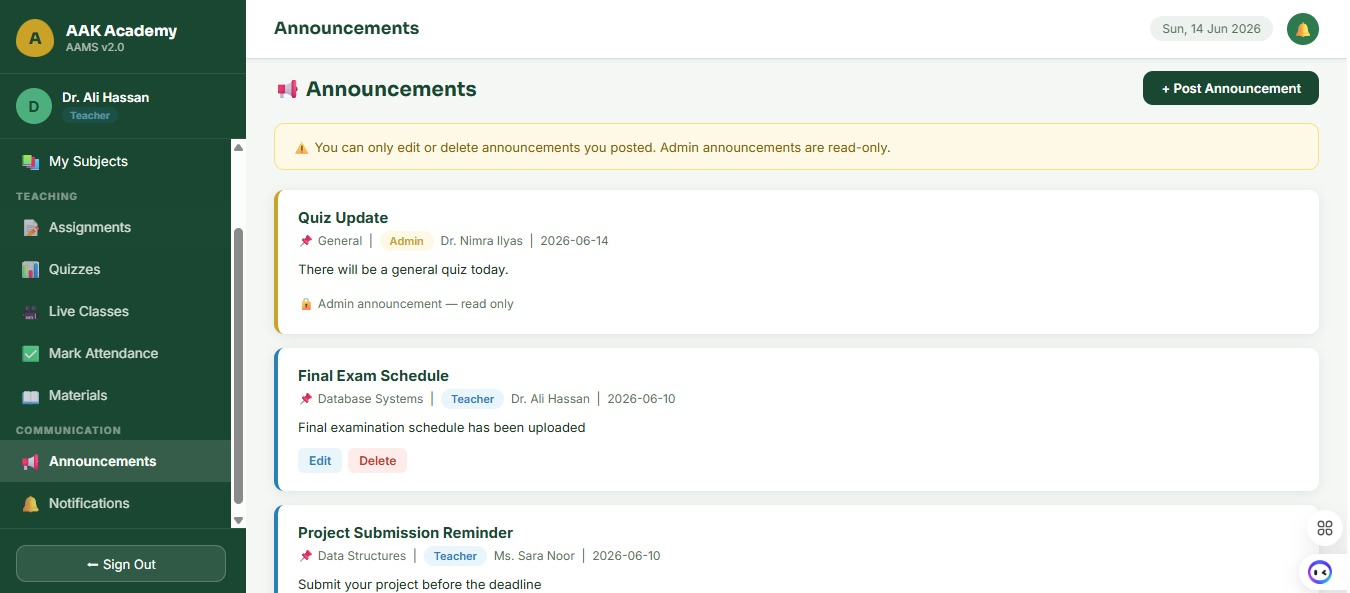
\includegraphics[width=0.8\linewidth]{teacherannouncement.png}
    \label{fig:placeholder}
\end{figure}
\caption{Teacher Announcements}
\end{figure}

\begin{figure}[H]
\centering
\includegraphics[width=\textwidth]{}
\begin{figure}
    \centering
    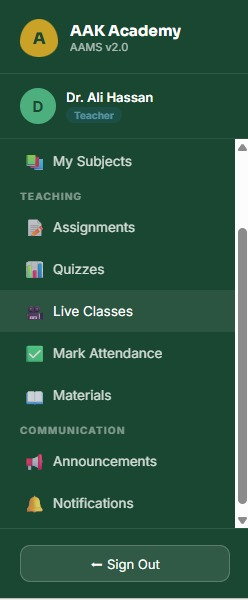
\includegraphics[width=0.3\linewidth]{teachermainfunc.png}
    \label{fig:placeholder}
\end{figure}
\caption{Teacher Main Functionalities}
\end{figure}

\clearpage

% ============================================================
% STUDENT MODULE
% ============================================================

\subsubsection*{Student Module}

\begin{figure}[H]
\centering
\includegraphics[width=\textwidth]{}
\begin{figure}
    \centering
    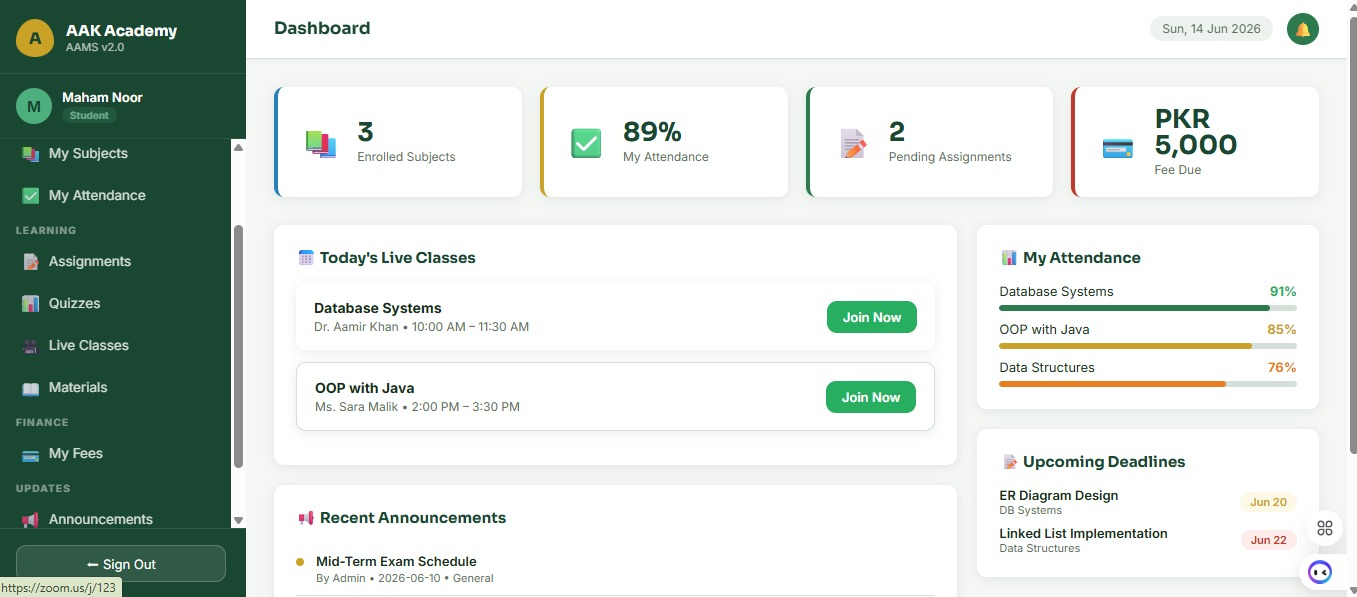
\includegraphics[width=0.8\linewidth]{studentmaindashboard.png}
    \label{fig:placeholder}
\end{figure}
\caption{Student Main Dashboard}
\end{figure}

\begin{figure}[H]
\centering
\includegraphics[width=\textwidth]{}
\begin{figure}
    \centering
    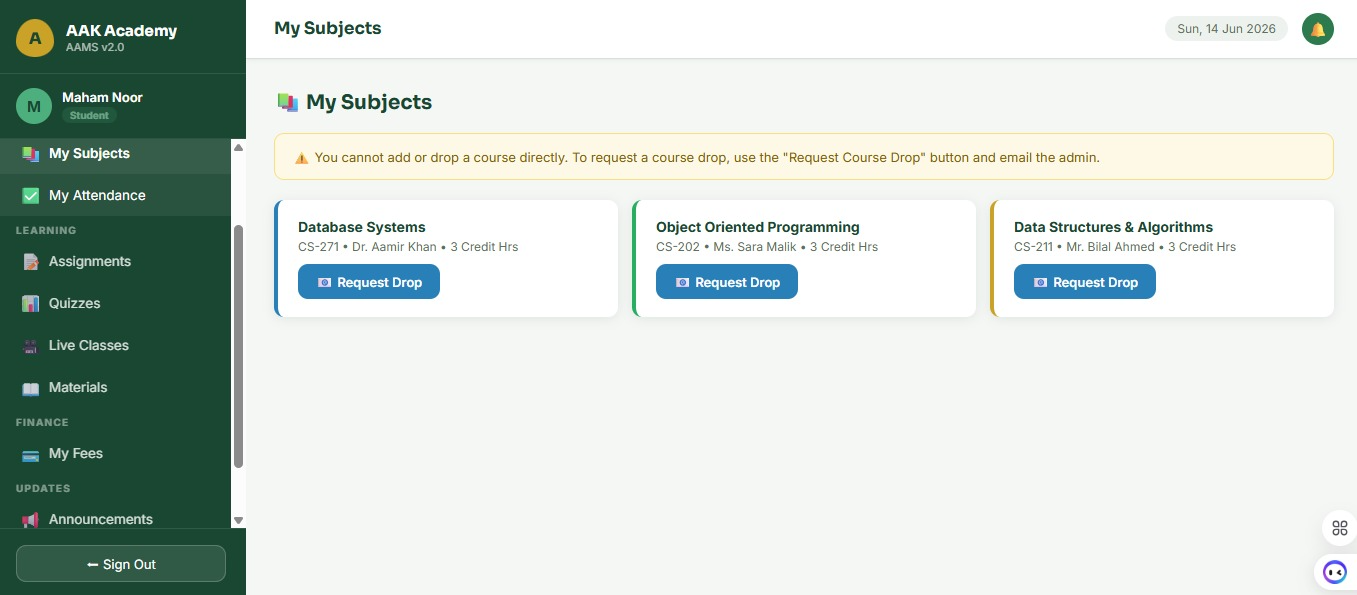
\includegraphics[width=0.8\linewidth]{studentsubjectsec.png}
  
    \label{fig:placeholder}
\end{figure}
\caption{Student Subject Section}
\end{figure}

\begin{figure}[H]
\centering
\includegraphics[width=\textwidth]{}
\begin{figure}
    \centering
    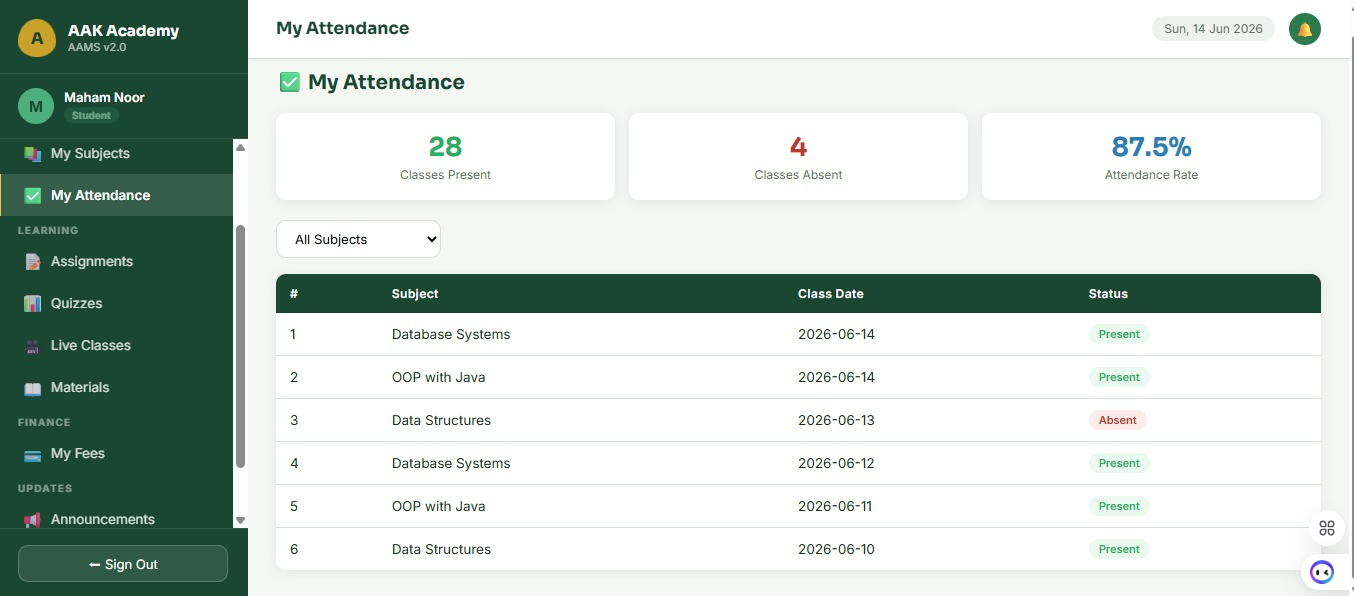
\includegraphics[width=0.8\linewidth]{studentattendence.png}
    \label{fig:placeholder}
\end{figure}
\caption{Student Attendance Section}
\end{figure}

\begin{figure}[H]
\centering
\includegraphics[width=\textwidth]{}
\begin{figure}
    \centering
    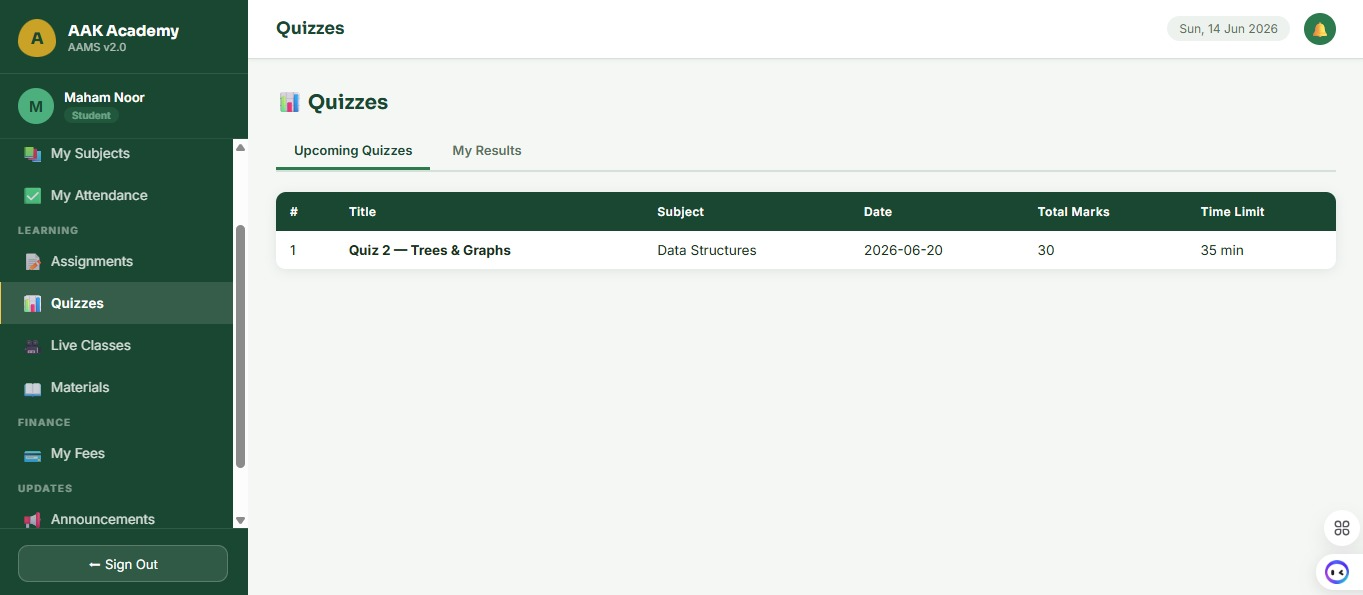
\includegraphics[width=0.8\linewidth]{studentquiz.png}
    \label{fig:placeholder}
\end{figure}
\caption{Student Quiz Section}
\end{figure}

\begin{figure}[H]
\centering
\includegraphics[width=\textwidth]{}
\begin{figure}
    \centering
    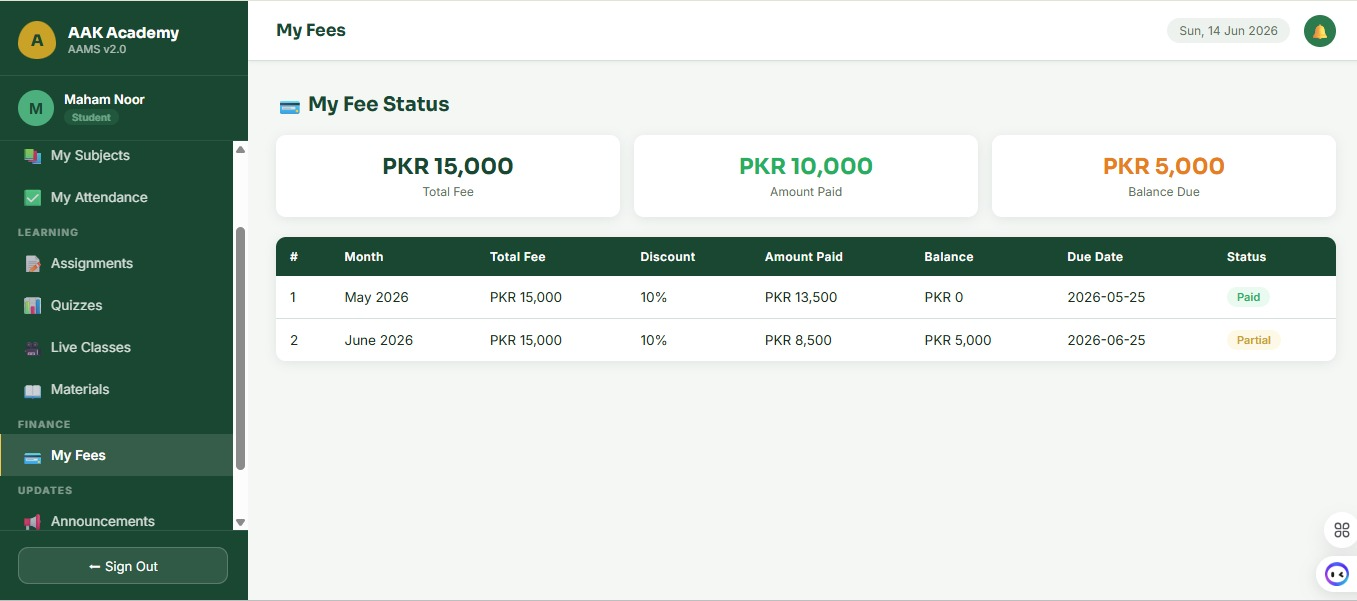
\includegraphics[width=0.8\linewidth]{studentfee.png}
    \label{fig:placeholder}
\end{figure}
\caption{Student Fee Section}
\end{figure}

\begin{figure}[H]
\centering
\includegraphics[width=\textwidth]{}
\begin{figure}
    \centering
    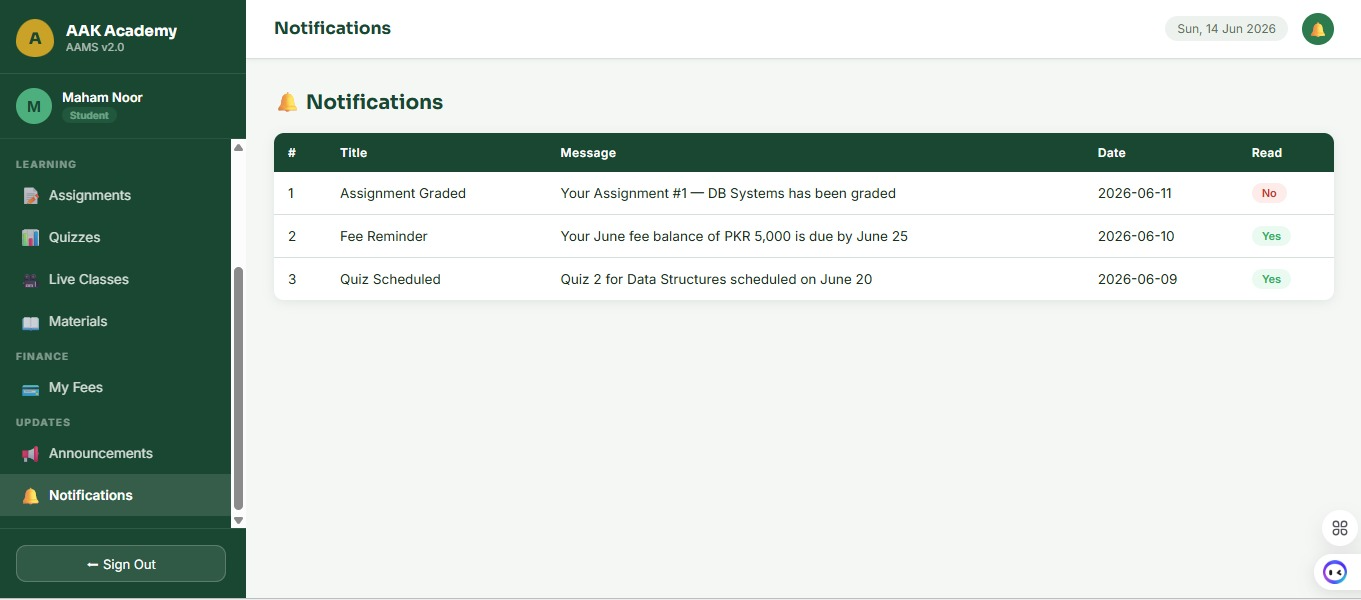
\includegraphics[width=0.8\linewidth]{studentnotificationpanel.png}
    \label{fig:placeholder}
\end{figure}
\caption{Student Notification Panel}
\end{figure}

\begin{figure}[H]
\centering
\includegraphics[width=\textwidth]{}
\begin{figure}
    \centering
    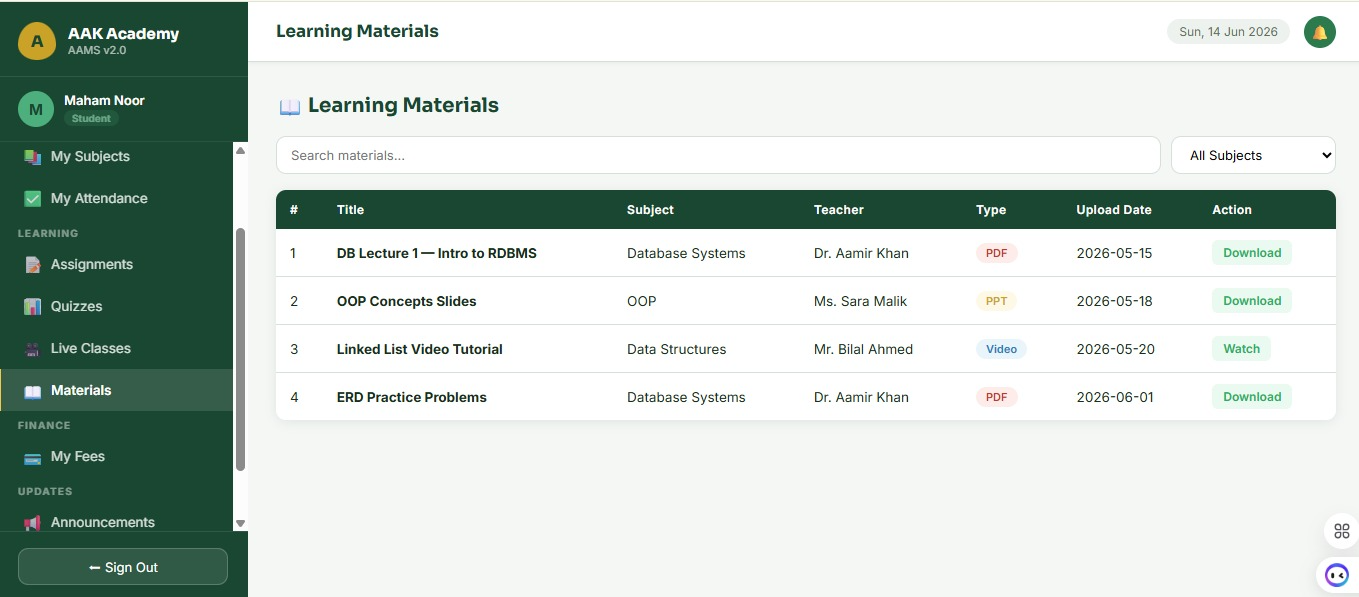
\includegraphics[width=0.8\linewidth]{studentlearningmaterial.png}
    \label{fig:placeholder}
\end{figure}
\caption{Student Learning Materials}
\end{figure}

\begin{figure}[H]
\centering
\includegraphics[width=\textwidth]{}
\begin{figure}
    \centering
    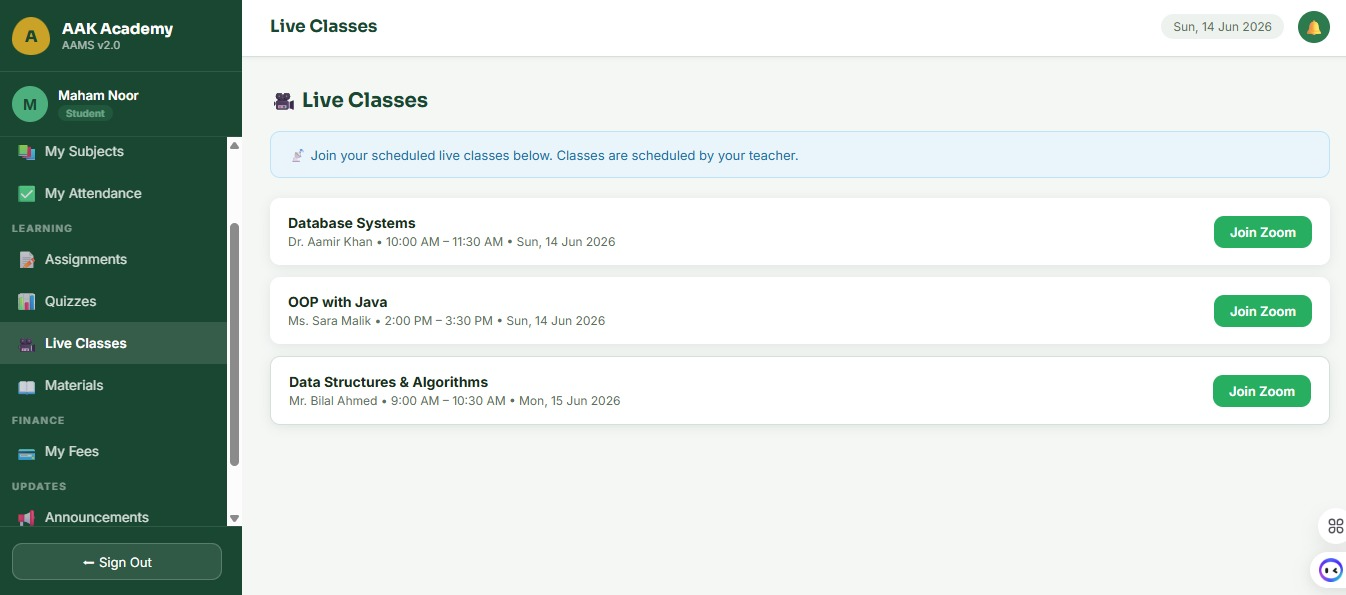
\includegraphics[width=0.8\linewidth]{liveclass student.png}
    \label{fig:placeholder}
\end{figure}
\caption{Student Live Classes}
\end{figure}

% ============================================================
%  TESTING
% ============================================================
\chapter*{TESTING \& VALIDATION}
\addcontentsline{toc}{chapter}{Testing \& Validation}

\section*{Database Connectivity Tests}

\begin{longtable}{|L{3.5cm}|L{4cm}|L{4cm}|C{2cm}|}
\hline
\textbf{Test} & \textbf{Action} & \textbf{Expected Result} & \textbf{Status} \\
\hline
\endfirsthead
\hline
\textbf{Test} & \textbf{Action} & \textbf{Expected Result} & \textbf{Status} \\
\hline
\endhead
Health check & GET /api/health & \{``ok'': true\} & \checkmark Pass \\
\hline
Login — Admin & POST /api/login & Returns object with admin\_id & \checkmark Pass \\
\hline
Login — Teacher & POST /api/login & Returns object with teacher\_id & \checkmark Pass \\
\hline
Login — Student & POST /api/login & Returns object with student\_id & \checkmark Pass \\
\hline
\end{longtable}

\section*{CRUD Operations}

\begin{longtable}{|L{3.5cm}|C{2cm}|C{2cm}|C{2cm}|C{2cm}|}
\hline
\textbf{Entity} & \textbf{Create} & \textbf{Read} & \textbf{Update} & \textbf{Delete} \\
\hline
\endfirsthead
\hline
\textbf{Entity} & \textbf{Create} & \textbf{Read} & \textbf{Update} & \textbf{Delete} \\
\hline
\endhead
Programs & \checkmark & \checkmark & \checkmark & \checkmark \\
\hline
Students & \checkmark & \checkmark & \checkmark & \checkmark \\
\hline
Teachers & \checkmark & \checkmark & \checkmark & \checkmark \\
\hline
Subjects & \checkmark & \checkmark & \checkmark & \checkmark \\
\hline
Enrollment & \checkmark & \checkmark & \checkmark & \checkmark \\
\hline
Fees & \checkmark & \checkmark & \checkmark & \checkmark \\
\hline
Announcements & \checkmark & \checkmark & \checkmark & \checkmark \\
\hline
\end{longtable}

\section*{Referential Integrity Tests}

\begin{longtable}{|L{3.5cm}|L{3.5cm}|L{4cm}|C{2cm}|}
\hline
\textbf{Test Case} & \textbf{Action} & \textbf{Expected} & \textbf{Status} \\
\hline
\endfirsthead
\hline
\textbf{Test Case} & \textbf{Action} & \textbf{Expected} & \textbf{Status} \\
\hline
\endhead
Delete user & DELETE user record & Cascades to admin/teacher/student & \checkmark Pass \\
\hline
Delete student & DELETE student & Cascades enrollment, fee\_record, attendance & \checkmark Pass \\
\hline
Delete program & DELETE program & Sets program\_id = NULL in student/subject & \checkmark Pass \\
\hline
Invalid enrollment & Enroll without valid student\_id & FK constraint error raised & \checkmark Pass \\
\hline
\end{longtable}

% ============================================================
%  CONCLUSION
% ============================================================
\chapter*{CONCLUSION}
\addcontentsline{toc}{chapter}{Conclusion}

The AAK Academy Management System successfully implements a \textbf{complete database-driven web application} that addresses the core challenges of manual academic management. The key achievements of this project are:

\begin{enumerate}[noitemsep]
    \item A \textbf{normalized 20-table relational schema} satisfying 3NF and BCNF across all entities.
    \item \textbf{Full ERD-to-relational mapping} with proper FK constraints, cascade rules, and performance indexes.
    \item A \textbf{role-based GUI} supporting Admin (17 pages), Teacher (8 pages), and Student (9 pages) workflows.
    \item \textbf{Real-time database connectivity} via a Node.js/Express REST API with a connection pool.
    \item \textbf{Complete CRUD operations} persisting immediately to MySQL with referential integrity.
    \item \textbf{Automated database programmability} via stored procedures and triggers.
    \item \textbf{Sample data} covering 400+ records across all 20 tables for all major academic and financial workflows.
\end{enumerate}

The three-tier architecture (Presentation $\rightarrow$ Application $\rightarrow$ Data) ensures clean separation of concerns, maintainability, and scalability. The system can be extended in future with features such as file upload handling, email notifications, automated report generation, and enhanced stored procedures for complex business logic.

% ============================================================
%  REFERENCES
% ============================================================
\chapter*{REFERENCES}
\addcontentsline{toc}{chapter}{References}

\begin{enumerate}[label={[\arabic*]}, noitemsep]
    \item R. Elmasri and S. Navathe, \textit{Fundamentals of Database Systems}, 7th ed. Pearson Education, 2015.
    \item C. J. Date, \textit{An Introduction to Database Systems}, 8th ed. Addison-Wesley, 2003.
    \item MySQL AB, \textit{MySQL 8.0 Reference Manual}. Oracle Corporation, 2023. [Online]. Available: \url{https://dev.mysql.com/doc/refman/8.0/en/}
    \item Node.js Foundation, \textit{Node.js Documentation}. [Online]. Available: \url{https://nodejs.org/en/docs/}
    \item Express.js, \textit{Express 4.x API Reference}. [Online]. Available: \url{https://expressjs.com/en/4x/api.html}
    \item npm, \textit{mysql2 package documentation}. [Online]. Available: \url{https://www.npmjs.com/package/mysql2}
\end{enumerate}

% ============================================================
%  APPENDIX
% ============================================================
\chapter*{APPENDIX: AI USAGE AND PROMPTS}
\addcontentsline{toc}{chapter}{Appendix: AI Usage and Prompts}

This section documents the use of AI tools during the development of this project.

\begin{longtable}{|C{0.8cm}|L{5cm}|L{4cm}|L{4.5cm}|}
\hline
\textbf{\#} & \textbf{Prompt Used} & \textbf{Tool} & \textbf{Purpose} \\
\hline
\endfirsthead
\hline
\textbf{\#} & \textbf{Prompt Used} & \textbf{Tool} & \textbf{Purpose} \\
\hline
\endhead
1 & ``Convert this ERD into a relational schema'' & Google Gemini & Converting the ERD diagram into structured relational schema notation \\
\hline
2 & [Add your prompts here] & [Tool name] & [Purpose] \\
\hline
3 & [Add your prompts here] & [Tool name] & [Purpose] \\
\hline
\end{longtable}

\subsection*{Appendix A: How to Run the Project}

\begin{lstlisting}[language=bash, caption={Setup and run commands}]
# Step 1: Navigate to project folder
cd "d:\4th Semester\DB\aakc"

# Step 2: Install Node.js dependencies
npm install

# Step 3: Setup database (requires MySQL running)
node setup-db.js Namal.123

# Step 4: Start the application server
npm start

# Step 5: Open browser and navigate to:
# http://localhost:3000
\end{lstlisting}

\subsection*{Appendix B: Project Directory Structure}

\begin{lstlisting}[caption={Project files and folders}]
aakc/
|-- AAMS_RoleBased.html      # Frontend GUI (role-based)
|-- server.js                # Express REST API server
|-- setup-db.js              # Automated database setup script
|-- dbDDL.sql                # Schema (CREATE TABLE statements)
|-- dbDML.sql                # Sample data (INSERT statements)
|-- package.json             # Node.js configuration
|-- .env                     # Environment variables (DB credentials)
|-- .gitignore               # Git ignore rules
`-- screenshots/             # Screenshots folder
    |-- 01_login.png
    |-- 02_admin_dashboard.png
    `-- ...
\end{lstlisting}

\subsection*{Appendix C: Login Credentials (Test Accounts)}

\begin{longtable}{|L{3cm}|L{5.5cm}|L{4cm}|}
\hline
\textbf{Role} & \textbf{Email} & \textbf{Password} \\
\hline
Admin & admin@aakacademy.pk & password123 \\
\hline
Teacher & ali.hassan@aakacademy.pk & password123 \\
\hline
Student & ahmed.raza@student.aakacademy.pk & password123 \\
\hline
Student & fatima.malik@student.aakacademy.pk & password123 \\
\hline
\end{longtable}

\subsection*{Appendix D: Entity Count Summary}

\begin{itemize}[noitemsep]
    \item \textbf{Total Entities (Tables):} 20
    \item \textbf{Total Foreign Key Relationships:} 35+
    \item \textbf{Total Performance Indexes:} 10
    \item \textbf{Total Sample Records:} 400+
\end{itemize}

\vfill
\begin{center}
\textit{Report prepared for Database Systems course --- Namal University --- June 2026}
\end{center}

\end{document}